\FPset\bc{30}
\FPset\hc{65}
\FPeval{\Ag}{round(\bc*\hc,2)}
\FPset\nvc{12}
\FPeval{\Ast}{round(\nvc*1.98,2)}
\FPeval{\pn}{round(0.8*0.7*(0.85*\fc*(\Ag-\Ast)+\fy*\Ast)/1000,2)}
\subsection{Diseño de columnas}
\noindent Se diseñara la columna del eje A con intersección del eje 5:\\
\noindent Geometría de la columna:
\begin{itemize}
  \item Ancho: $b=\bc \mathrm{~cm}$
  \item Peralte: $h=\hc \mathrm{~cm}$
\end{itemize}
\noindent
Datos de los materiales:\\
\noindent Igual que los definidos para el diseño de vigas.\\
Datos del refuerzo:
\begin{itemize}
  \item Recubrimiento: $r_{e}=4 \mathrm{~cm}$
  \item Diámetro del acero longitudinal: $d_{b}=5/8"$
  \item Diámetro de estribos: $d_{e}=3/8"$
\end{itemize}
\subsubsection{Factores de minoración}
\begin{itemize}
  \item Según el artículo 9.3.2.2 el factor de minoración para compresión es $\phi_{\text {com }}=0,70$

  \item Según el artículo 9.3.2.2 el factor de minoración para flexocompresión $\phi$ puede incrementarse linealmente hasta 0,90 en la medida que $\phi P_{n}$ disminuye desde $0,1 \cdot f_{c}^{\prime} A_{g}$ o $\phi P_{b}$, el que sea menor, hasta cero.
\end{itemize}

\subsubsection{Diseño por flexión y carga axial (Capítulo 10)}
\noindent
Como se menciona en 21.5.1.1 y 21.6.1.1 un elemento es considerado como columna cuando la carga axial amplificada en compresión $P_{u}$ excede $0,1 \cdot f_{c}^{\prime} A_{g}$.\\
La cuantía mínima para elementos en compresión según el artículo 10.9.1 no debe ser menor que $1 \%$.\\
La resistencia máxima de diseño a compresión Ecu. 10-2 de E-060 sera:
\begin{align}
\phi P_{n}=0,80 \cdot \phi_{c o m} \cdot\left[0,85 \cdot f_{c}^{\prime} \cdot\left(A_{g}-A_{s t}\right)+f_{y} \cdot A_{s t}\right]
\end{align}
\begin{figure}[h!]
    \centering
    \caption{Distribución de esfuerzos y deformaciones en una columna}
    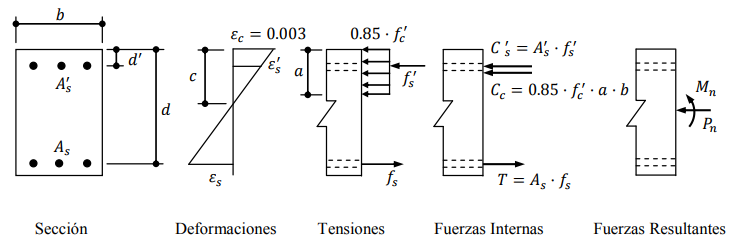
\includegraphics[scale=0.67]{IMAGENES/c1.PNG}
    \caption*{\small Fuente: \it \cite{cordova2015}}
    \label{vig}
\end{figure}
\newpage
\begin{figure}[ht!]
    \centering
    \caption{Diagrama de interacción en una columna}
    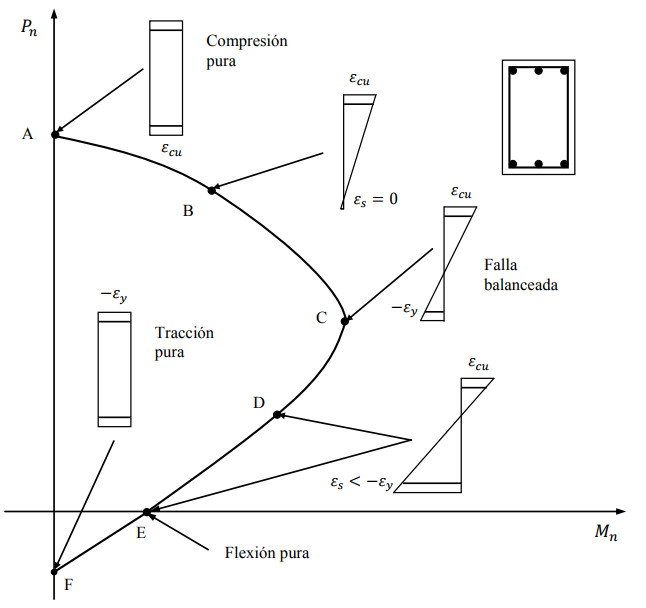
\includegraphics[scale=0.67]{IMAGENES/c2.PNG}
    \caption*{\small Fuente: \it \cite{cordova2015}}
    \label{vig}
\end{figure}
\noindent Preliminarmente se considerara $\nvc$ varillas de 5/8", lo cual cumple con la cuantía mínima del 1\%.\\
Capacidad máxima a carga axial de la columna.
\begin{align*}
\phi P_{n}=0,80 \cdot 0,70 \cdot\left[0,85 \cdot \fc \cdot\left(\Ag-\Ast\right)+\fy \cdot \Ast\right]=\pn \mathrm{~ton}
\end{align*}
\newpage
\begin{figure}[h!]
    \centering
    \subfigure[Eje débil]{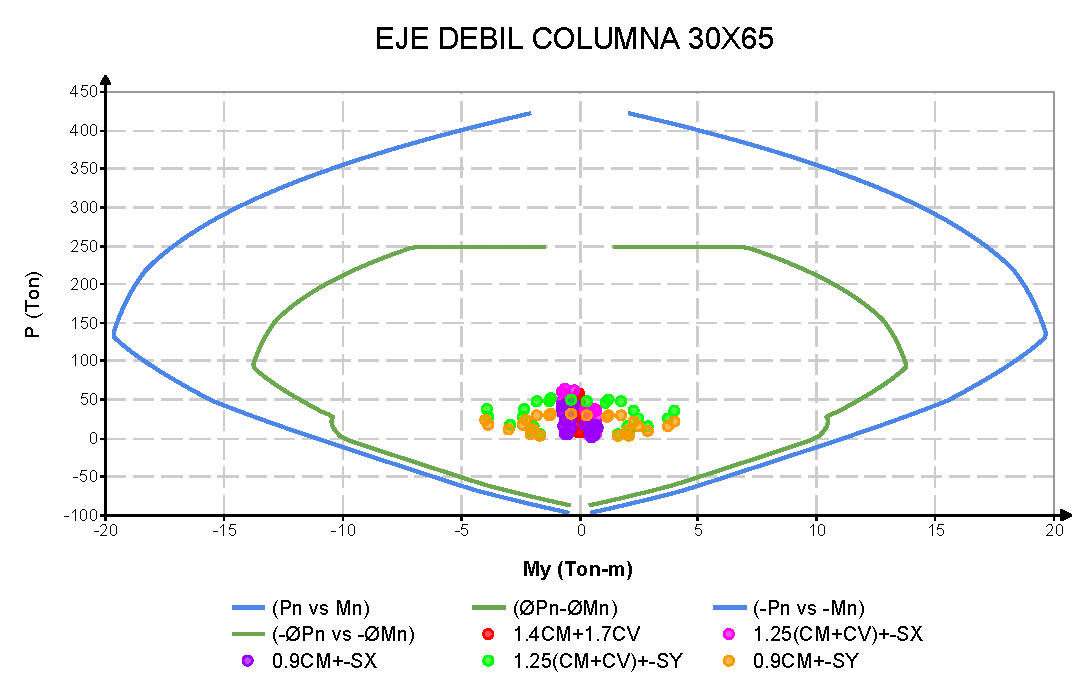
\includegraphics[width=150mm]{IMAGENES/colx.pdf}}\hspace{0mm}
    \subfigure[Eje fuerte]{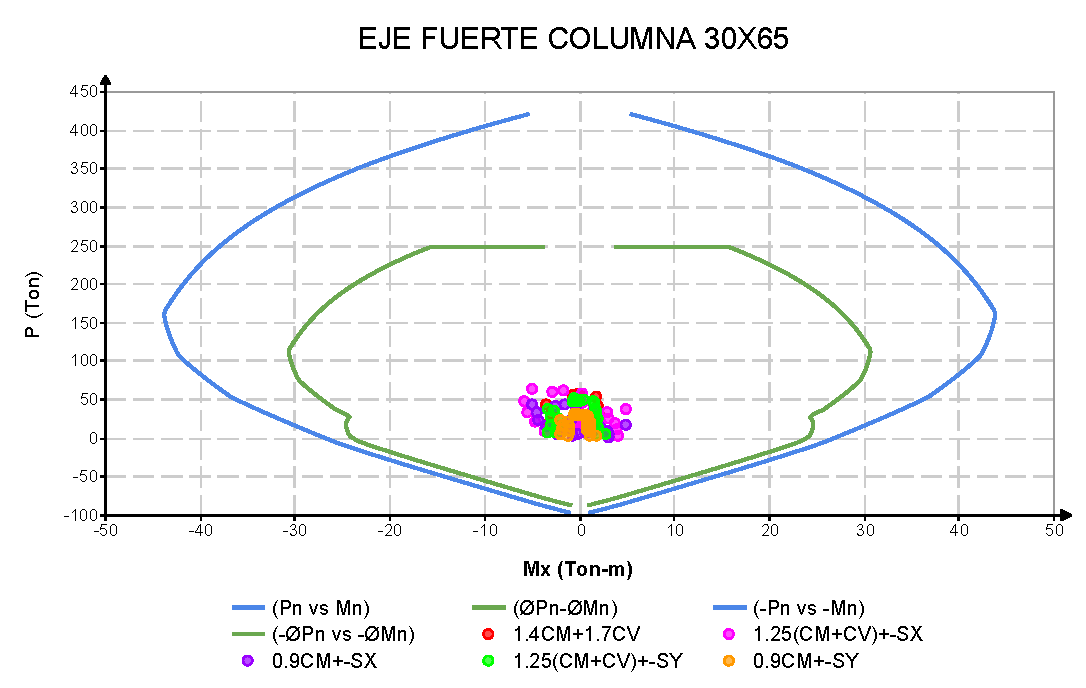
\includegraphics[width=150mm]{IMAGENES/coly.pdf}}
    \caption{Diagrama de interacción de la columna C-1 30x65 cm}
    \label{reqv}
\end{figure}

\begin{figure}[ht!]
    \centering
    \caption{Corte por capacidad en columnas}
    \subfigure[Fuerza cortante de columnas en sistemas de muros ]{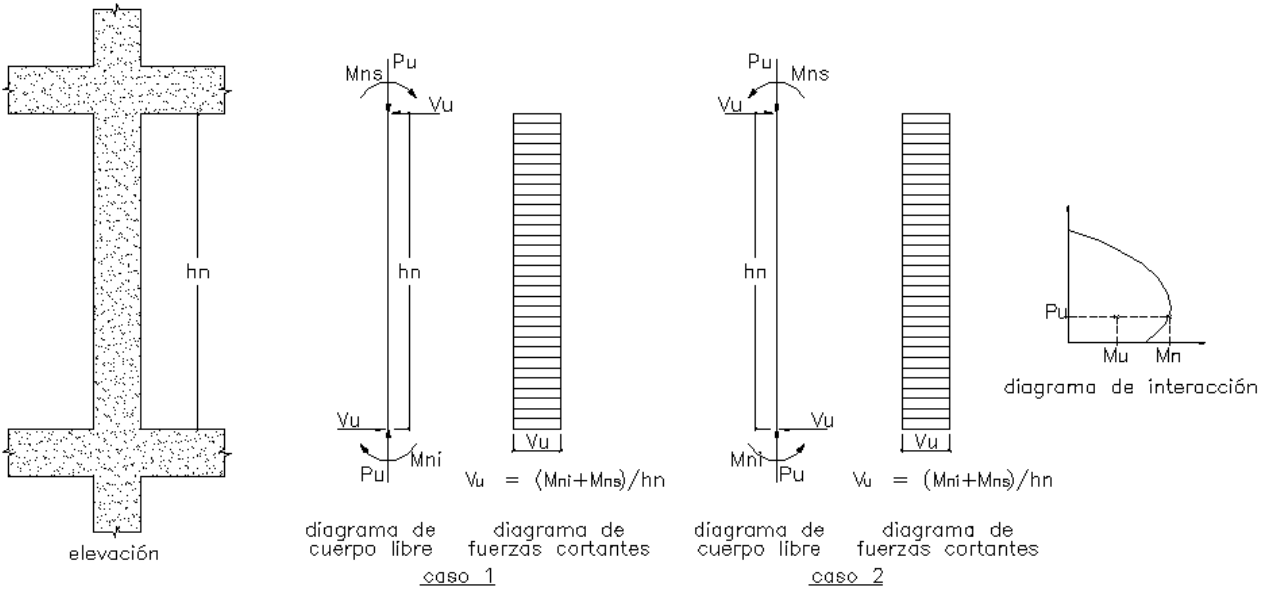
\includegraphics[width=150mm]{IMAGENES/colm.PNG}}\hspace{0mm}
    \subfigure[Fuerza cortante de columnas en sistemas duales o aporticados]{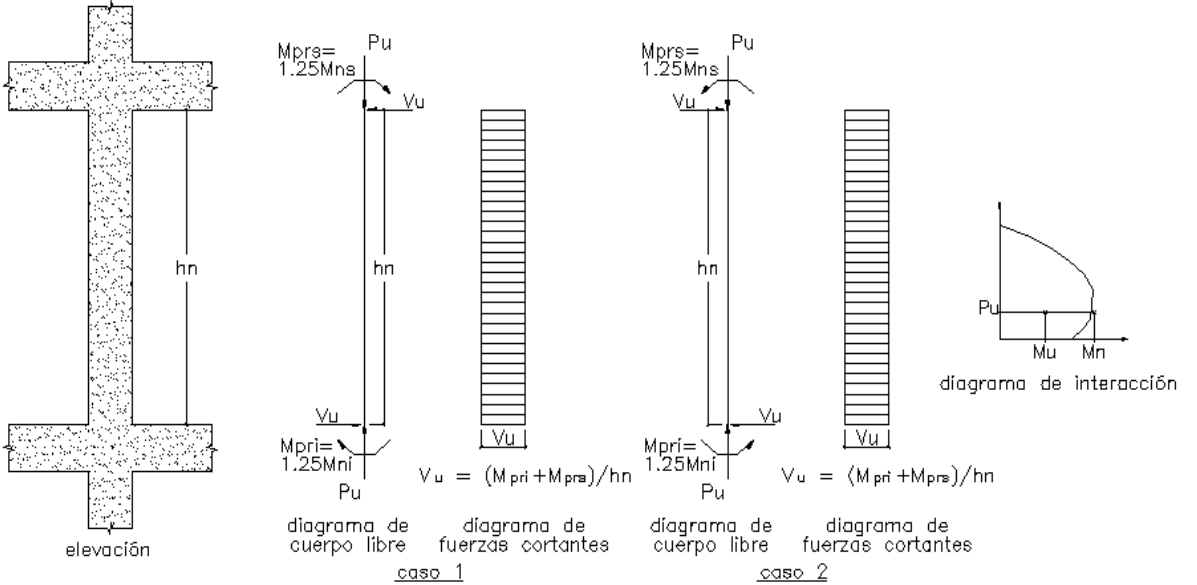
\includegraphics[width=150mm]{IMAGENES/colp.PNG}}
    \caption*{\small Fuente: \it \cite{E-060}}
    \label{reqv}
\end{figure}
\begin{align}
V_{u,1}=\frac{M_{n i}+M_{n s}}{h_{n}}\label{vcap1}\\
V_{u,2}=\frac{M_{p i}+M_{p s}}{h_{n}}\label{vcap2}
\end{align}
\newpage
\noindent
Donde:\\
$V_{u,1}$: Cortante en columnas, sistema de muros\\
$V_{u,2}$: Cortante en columnas, sistema de pórticos\\
$M_{n i}, M_{n s}$: Momentos nominales inferior e superior de la columna\\
$M_{p i}, M_{p s}$: Momentos probables inferior e superior de la columna\\

\subsubsection{Resistencia a corte Cap. 11}
La resistencia a cortante del concreto en una columna en compresión y tracción, esta dado respectivamente por:
\begin{flalign}
&\textup{Ecu.(11.4) E-060:}&\phi V_{c}&=\phi_{c} \cdot 0,53 \cdot \sqrt{f_{c}^{\prime}} \cdot b \cdot d \cdot\left(1+\frac{N_{u}}{140 \cdot A_{g}}\right)&&\label{vc1}\\
&\textup{Ecu.(11.8) E-060:}&\phi V_{c}&=\phi_{c} \cdot 0,53 \cdot \sqrt{f_{c}^{\prime}} \cdot b \cdot d \cdot\left(1-\frac{N_{u}}{35 \cdot A_{g}}\right)\label{vc2}
\end{flalign}
\noindent
Donde:\\
$N_{u}:$ Es la carga axial\\
$A_{g}:$ Es el área bruta de la sección\\
$d:$ Peralte efectivo en la dirección de análisis\\
$b:$ Ancho de la columna en la dirección de análisis\\
\noindent Los peraltes efectivos en las direcciones fuerte y débil de la columna serán:
\FPset\rec{4}
\FPeval{\dest}{round(3*2.54/8,2)}
\FPeval{\dvarc}{round(5*2.54/8,2)}
\FPeval{\defecx}{round(\hc-\rec-\dest-\dvarc/2,2)}
\FPeval{\defecy}{round(\bc-\rec-\dest-\dvarc/2,2)}
\FPeval{\vmaxx}{round(2.1*\rc*\hc*\defecx/1000,2)}
\FPeval{\vmaxy}{round(2.1*\rc*\bc*\defecy/1000,2)}
\begin{flalign*}
d_{x}=h_{c}-r_{e}-d_{e}-d_{b}/2&=\hc-\rec-\dest-\dvarc/2=\defecx \mathrm{~cm}\\
d_{y}=b_{c}-r_{e}-d_{e}-d_{b}/2&=\bc-\rec-\dest-\dvarc/2=\defecy \mathrm{~cm}
\end{flalign*}
\noindent La máxima capacidad de los estribos a corte en las direcciones fuerte y débil de la columna según la ecuación \ref{vmax} serán:
\begin{flalign*}
V_{ex, \max }&=2,1 \cdot \sqrt{\fc} \cdot \hc \cdot \defecx=\vmaxx \mathrm{ton}\\
V_{ey, \max }&=2,1 \cdot \sqrt{\fc} \cdot \bc \cdot \defecy=\vmaxy \mathrm{ton}
\end{flalign*}
\newpage
\begin{table}[ht!]
  \centering
  \caption{Diseño por capacidad en columnas (a)}
    {
\extrarowheight = 0ex
\renewcommand{\arraystretch}{1.2}
\begin{tabular}{*{2}{>{\centering\arraybackslash}m{0.8cm}}*{3}{|>{\centering\arraybackslash}m{1.5cm}}*{3}{|>{\centering\arraybackslash}m{1cm}}*{1}{|>{\centering\arraybackslash}m{1.1cm}}*{1}{|>{\centering\arraybackslash}m{1cm}}|}
\hline
\multicolumn{10}{|c|}{\textit{\textbf{1.25(CM+CV)+SX}}}                                                                                                                                                                                                          \\ \hline
\multicolumn{1}{|c|}{\multirow{2}{*}{\textbf{Piso}}} & \multicolumn{1}{c|}{(1)}            & \multicolumn{1}{c|}{(2)}               & \multicolumn{1}{c|}{(3)}            & \multicolumn{1}{c|}{(4)}                & \multicolumn{1}{c|}{(5)}                    & \multicolumn{1}{c|}{(6)}                    & \multicolumn{1}{c|}{(7)}                    & \multicolumn{1}{c|}{(8)}                & (9)                    \\ \cline{2-10} 
\multicolumn{1}{|c|}{}                               & \textbf{h (m)} & \textbf{Pu (ton)} & \textbf{a (cm)} & \textbf{Mn (ton.m)} & \textbf{Vu (ton)}     & \textbf{$\phi$Vc (ton)}    & \textbf{Ve}          & \textbf{ramas}    & \textbf{s (cm)}        \\ \hline
\multicolumn{1}{|c|}{\multirow{2}{*}{5}}             & \multicolumn{1}{c|}{2.2}            & \multicolumn{1}{c|}{-7.44}             & \multicolumn{1}{c|}{10.76}          & \multicolumn{1}{c|}{28.11}              & \multicolumn{1}{c|}{\multirow{2}{*}{25.67}} & \multicolumn{1}{c|}{\multirow{2}{*}{11.92}} & \multicolumn{1}{c|}{\multirow{2}{*}{16.17}} & \multicolumn{1}{c|}{\multirow{2}{*}{3}} & \multirow{2}{*}{32.89} \\ \cline{2-5}
\multicolumn{1}{|c|}{}                               & \multicolumn{1}{c|}{0}              & \multicolumn{1}{c|}{-8.73}             & \multicolumn{1}{c|}{10.89}          & \multicolumn{1}{c|}{28.37}              & \multicolumn{1}{c|}{}                       & \multicolumn{1}{c|}{}                       & \multicolumn{1}{c|}{}                       & \multicolumn{1}{c|}{}                   &                        \\ \hline
\multicolumn{1}{|c|}{\multirow{2}{*}{4}}             & \multicolumn{1}{c|}{2.2}            & \multicolumn{1}{c|}{-19.93}            & \multicolumn{1}{c|}{12.05}          & \multicolumn{1}{c|}{30.54}              & \multicolumn{1}{c|}{\multirow{2}{*}{27.88}} & \multicolumn{1}{c|}{\multirow{2}{*}{12.45}} & \multicolumn{1}{c|}{\multirow{2}{*}{18.14}} & \multicolumn{1}{c|}{\multirow{2}{*}{3}} & \multirow{2}{*}{29.32} \\ \cline{2-5}
\multicolumn{1}{|c|}{}                               & \multicolumn{1}{c|}{0}              & \multicolumn{1}{c|}{-21.22}            & \multicolumn{1}{c|}{12.19}          & \multicolumn{1}{c|}{30.79}              & \multicolumn{1}{c|}{}                       & \multicolumn{1}{c|}{}                       & \multicolumn{1}{c|}{}                       & \multicolumn{1}{c|}{}                   &                        \\ \hline
\multicolumn{1}{|c|}{\multirow{2}{*}{3}}             & \multicolumn{1}{c|}{2.2}            & \multicolumn{1}{c|}{-32.94}            & \multicolumn{1}{c|}{13.53}          & \multicolumn{1}{c|}{32.99}              & \multicolumn{1}{c|}{\multirow{2}{*}{30.11}} & \multicolumn{1}{c|}{\multirow{2}{*}{13.01}} & \multicolumn{1}{c|}{\multirow{2}{*}{20.12}} & \multicolumn{1}{c|}{\multirow{2}{*}{3}} & \multirow{2}{*}{26.44} \\ \cline{2-5}
\multicolumn{1}{|c|}{}                               & \multicolumn{1}{c|}{0}              & \multicolumn{1}{c|}{-34.23}            & \multicolumn{1}{c|}{13.69}          & \multicolumn{1}{c|}{33.24}              & \multicolumn{1}{c|}{}                       & \multicolumn{1}{c|}{}                       & \multicolumn{1}{c|}{}                       & \multicolumn{1}{c|}{}                   &                        \\ \hline
\multicolumn{1}{|c|}{\multirow{2}{*}{2}}             & \multicolumn{1}{c|}{2.2}            & \multicolumn{1}{c|}{-46.19}            & \multicolumn{1}{c|}{15.17}          & \multicolumn{1}{c|}{35.37}              & \multicolumn{1}{c|}{\multirow{2}{*}{32.26}} & \multicolumn{1}{c|}{\multirow{2}{*}{13.57}} & \multicolumn{1}{c|}{\multirow{2}{*}{21.99}} & \multicolumn{1}{c|}{\multirow{2}{*}{3}} & \multirow{2}{*}{24.19} \\ \cline{2-5}
\multicolumn{1}{|c|}{}                               & \multicolumn{1}{c|}{0}              & \multicolumn{1}{c|}{-47.47}            & \multicolumn{1}{c|}{15.34}          & \multicolumn{1}{c|}{35.60}              & \multicolumn{1}{c|}{}                       & \multicolumn{1}{c|}{}                       & \multicolumn{1}{c|}{}                       & \multicolumn{1}{c|}{}                   &                        \\ \hline
\multicolumn{1}{|c|}{\multirow{2}{*}{1}}             & \multicolumn{1}{c|}{2.8}            & \multicolumn{1}{c|}{-59.25}            & \multicolumn{1}{c|}{16.78}          & \multicolumn{1}{c|}{37.33}              & \multicolumn{1}{c|}{\multirow{2}{*}{26.73}} & \multicolumn{1}{c|}{\multirow{2}{*}{14.12}} & \multicolumn{1}{c|}{\multirow{2}{*}{14.83}} & \multicolumn{1}{c|}{\multirow{2}{*}{3}} & \multirow{2}{*}{35.86} \\ \cline{2-5}
\multicolumn{1}{|c|}{}                               & \multicolumn{1}{c|}{0}              & \multicolumn{1}{c|}{-60.88}            & \multicolumn{1}{c|}{16.96}          & \multicolumn{1}{c|}{37.52}              & \multicolumn{1}{c|}{}                       & \multicolumn{1}{c|}{}                       & \multicolumn{1}{c|}{}                       & \multicolumn{1}{c|}{}                   &                        \\ \hline
\multicolumn{1}{|c|}{\multirow{2}{*}{0}}             & \multicolumn{1}{c|}{2.15}           & \multicolumn{1}{c|}{-62.91}            & \multicolumn{1}{c|}{17.19}          & \multicolumn{1}{c|}{37.75}              & \multicolumn{1}{c|}{\multirow{2}{*}{35.18}} & \multicolumn{1}{c|}{\multirow{2}{*}{14.28}} & \multicolumn{1}{c|}{\multirow{2}{*}{24.59}} & \multicolumn{1}{c|}{\multirow{2}{*}{3}} & \multirow{2}{*}{21.64} \\ \cline{2-5}
\multicolumn{1}{|c|}{}                               & \multicolumn{1}{c|}{0}              & \multicolumn{1}{c|}{-64.17}            & \multicolumn{1}{c|}{17.33}          & \multicolumn{1}{c|}{37.89}              & \multicolumn{1}{c|}{}                       & \multicolumn{1}{c|}{}                       & \multicolumn{1}{c|}{}                       & \multicolumn{1}{c|}{}                   &                        \\ \hline
\end{tabular}
}
\end{table}
\vspace{0.5cm}
% Please add the following required packages to your document preamble:
% \usepackage{multirow}
\begin{table}[hb!]
  \centering
  \caption{Diseño por capacidad en columnas (b)}
    {
\extrarowheight = 0ex
\renewcommand{\arraystretch}{1.2}
\begin{tabular}{*{2}{>{\centering\arraybackslash}m{0.8cm}}*{3}{|>{\centering\arraybackslash}m{1.5cm}}*{3}{|>{\centering\arraybackslash}m{1cm}}*{1}{|>{\centering\arraybackslash}m{1.1cm}}*{1}{|>{\centering\arraybackslash}m{1cm}}|}
\hline
\multicolumn{10}{|c|}{\textit{\textbf{1.25(CM+CV)-SX}}}                                                                                                                                                                                                          \\ \hline
\multicolumn{1}{|c|}{\multirow{2}{*}{\textbf{Piso}}} & \multicolumn{1}{c|}{(1)}            & \multicolumn{1}{c|}{(2)}               & \multicolumn{1}{c|}{(3)}            & \multicolumn{1}{c|}{(4)}                & \multicolumn{1}{c|}{(5)}                    & \multicolumn{1}{c|}{(6)}                    & \multicolumn{1}{c|}{(7)}                    & \multicolumn{1}{c|}{(8)}                & (9)                    \\ \cline{2-10} 
\multicolumn{1}{|c|}{}                               & \textbf{h (m)} & \textbf{Pu (ton)} & \textbf{a (cm)} & \textbf{Mn (ton.m)} & \textbf{Vu (ton)}     & \textbf{$\phi$Vc (ton)}    & \textbf{Ve}          & \textbf{ramas}    & \textbf{s (cm)}        \\ \hline
\multicolumn{1}{|c|}{\multirow{2}{*}{5}}             & \multicolumn{1}{c|}{2.2}            & \multicolumn{1}{c|}{-4.22}             & \multicolumn{1}{c|}{10.45}           & \multicolumn{1}{c|}{27.47}               & \multicolumn{1}{c|}{\multirow{2}{*}{25.10}} & \multicolumn{1}{c|}{\multirow{2}{*}{11.78}} & \multicolumn{1}{c|}{\multirow{2}{*}{15.66}} & \multicolumn{1}{c|}{\multirow{2}{*}{3}} & \multirow{2}{*}{33.97} \\ \cline{2-5}
\multicolumn{1}{|c|}{}                               & \multicolumn{1}{c|}{0}              & \multicolumn{1}{c|}{-5.51}             & \multicolumn{1}{c|}{10.58}           & \multicolumn{1}{c|}{27.74}               & \multicolumn{1}{c|}{}                       & \multicolumn{1}{c|}{}                       & \multicolumn{1}{c|}{}                       & \multicolumn{1}{c|}{}                   &                        \\ \hline
\multicolumn{1}{|c|}{\multirow{2}{*}{4}}             & \multicolumn{1}{c|}{2.2}            & \multicolumn{1}{c|}{-11.91}            & \multicolumn{1}{c|}{11.21}           & \multicolumn{1}{c|}{28.99}               & \multicolumn{1}{c|}{\multirow{2}{*}{26.47}} & \multicolumn{1}{c|}{\multirow{2}{*}{12.11}} & \multicolumn{1}{c|}{\multirow{2}{*}{16.89}} & \multicolumn{1}{c|}{\multirow{2}{*}{3}} & \multirow{2}{*}{31.50} \\ \cline{2-5}
\multicolumn{1}{|c|}{}                               & \multicolumn{1}{c|}{0}              & \multicolumn{1}{c|}{-13.20}            & \multicolumn{1}{c|}{11.34}           & \multicolumn{1}{c|}{29.24}               & \multicolumn{1}{c|}{}                       & \multicolumn{1}{c|}{}                       & \multicolumn{1}{c|}{}                       & \multicolumn{1}{c|}{}                   &                        \\ \hline
\multicolumn{1}{|c|}{\multirow{2}{*}{3}}             & \multicolumn{1}{c|}{2.2}            & \multicolumn{1}{c|}{-19.16}            & \multicolumn{1}{c|}{11.97}           & \multicolumn{1}{c|}{30.40}               & \multicolumn{1}{c|}{\multirow{2}{*}{27.75}} & \multicolumn{1}{c|}{\multirow{2}{*}{12.42}} & \multicolumn{1}{c|}{\multirow{2}{*}{18.03}} & \multicolumn{1}{c|}{\multirow{2}{*}{3}} & \multirow{2}{*}{29.50} \\ \cline{2-5}
\multicolumn{1}{|c|}{}                               & \multicolumn{1}{c|}{0}              & \multicolumn{1}{c|}{-20.45}            & \multicolumn{1}{c|}{12.11}           & \multicolumn{1}{c|}{30.65}               & \multicolumn{1}{c|}{}                       & \multicolumn{1}{c|}{}                       & \multicolumn{1}{c|}{}                       & \multicolumn{1}{c|}{}                   &                        \\ \hline
\multicolumn{1}{|c|}{\multirow{2}{*}{2}}             & \multicolumn{1}{c|}{2.2}            & \multicolumn{1}{c|}{-26.38}            & \multicolumn{1}{c|}{12.77}           & \multicolumn{1}{c|}{31.77}               & \multicolumn{1}{c|}{\multirow{2}{*}{29.00}} & \multicolumn{1}{c|}{\multirow{2}{*}{12.73}} & \multicolumn{1}{c|}{\multirow{2}{*}{19.14}} & \multicolumn{1}{c|}{\multirow{2}{*}{3}} & \multirow{2}{*}{27.79} \\ \cline{2-5}
\multicolumn{1}{|c|}{}                               & \multicolumn{1}{c|}{0}              & \multicolumn{1}{c|}{-27.67}            & \multicolumn{1}{c|}{12.92}           & \multicolumn{1}{c|}{32.02}               & \multicolumn{1}{c|}{}                       & \multicolumn{1}{c|}{}                       & \multicolumn{1}{c|}{}                       & \multicolumn{1}{c|}{}                   &                        \\ \hline
\multicolumn{1}{|c|}{\multirow{2}{*}{1}}             & \multicolumn{1}{c|}{2.8}            & \multicolumn{1}{c|}{-34.02}          & \multicolumn{1}{c|}{13.66}           & \multicolumn{1}{c|}{33.19}           & \multicolumn{1}{c|}{\multirow{2}{*}{23.82}} & \multicolumn{1}{c|}{\multirow{2}{*}{13.05}} & \multicolumn{1}{c|}{\multirow{2}{*}{12.67}} & \multicolumn{1}{c|}{\multirow{2}{*}{3}} & \multirow{2}{*}{42.00} \\ \cline{2-5}
\multicolumn{1}{|c|}{}                               & \multicolumn{1}{c|}{0}              & \multicolumn{1}{c|}{-35.66}          & \multicolumn{1}{c|}{13.86}           & \multicolumn{1}{c|}{33.50}           & \multicolumn{1}{c|}{}                       & \multicolumn{1}{c|}{}                       & \multicolumn{1}{c|}{}                       & \multicolumn{1}{c|}{}                   &                        \\ \hline
\multicolumn{1}{|c|}{\multirow{2}{*}{0}}             & \multicolumn{1}{c|}{2.15}           & \multicolumn{1}{c|}{-35.97}            & \multicolumn{1}{c|}{13.90}           & \multicolumn{1}{c|}{33.56}               & \multicolumn{1}{c|}{\multirow{2}{*}{31.32}} & \multicolumn{1}{c|}{\multirow{2}{*}{13.13}} & \multicolumn{1}{c|}{\multirow{2}{*}{21.40}} & \multicolumn{1}{c|}{\multirow{2}{*}{3}} & \multirow{2}{*}{24.86} \\ \cline{2-5}
\multicolumn{1}{|c|}{}                               & \multicolumn{1}{c|}{0}              & \multicolumn{1}{c|}{-37.23}            & \multicolumn{1}{c|}{14.05}           & \multicolumn{1}{c|}{33.78}               & \multicolumn{1}{c|}{}                       & \multicolumn{1}{c|}{}                       & \multicolumn{1}{c|}{}                       & \multicolumn{1}{c|}{}                   &                        \\ \hline
\end{tabular}
}
\end{table}
\begin{table}[ht!]
  \centering
  \caption{Diseño por capacidad en columnas (c)}
    {
\extrarowheight = 0ex
\renewcommand{\arraystretch}{1.2}
\begin{tabular}{*{2}{>{\centering\arraybackslash}m{0.8cm}}*{3}{|>{\centering\arraybackslash}m{1.5cm}}*{3}{|>{\centering\arraybackslash}m{1cm}}*{1}{|>{\centering\arraybackslash}m{1.1cm}}*{1}{|>{\centering\arraybackslash}m{1cm}}|}
\hline
\multicolumn{10}{|c|}{\textit{\textbf{0.9CM+SX}}}                                                                                                                                                                                                          \\ \hline
\multicolumn{1}{|c|}{\multirow{2}{*}{\textbf{Piso}}} & \multicolumn{1}{c|}{(1)}            & \multicolumn{1}{c|}{(2)}               & \multicolumn{1}{c|}{(3)}            & \multicolumn{1}{c|}{(4)}                & \multicolumn{1}{c|}{(5)}                    & \multicolumn{1}{c|}{(6)}                    & \multicolumn{1}{c|}{(7)}                    & \multicolumn{1}{c|}{(8)}                & (9)                    \\ \cline{2-10} 
\multicolumn{1}{|c|}{}                               & \textbf{h (m)} & \textbf{Pu (ton)} & \textbf{a (cm)} & \textbf{Mn (ton.m)} & \textbf{Vu (Ton)}     & \textbf{$\phi$Vc (ton)}    & \textbf{Ve}          & \textbf{ramas}    & \textbf{s (cm)}        \\ \hline
\multicolumn{1}{|c|}{\multirow{2}{*}{5}}             & \multicolumn{1}{c|}{2.2}            & \multicolumn{1}{c|}{-5.30}             & \multicolumn{1}{c|}{10.56}          & \multicolumn{1}{c|}{27.70}              & \multicolumn{1}{c|}{\multirow{2}{*}{25.26}} & \multicolumn{1}{c|}{\multirow{2}{*}{11.83}} & \multicolumn{1}{c|}{\multirow{2}{*}{15.80}} & \multicolumn{1}{c|}{\multirow{2}{*}{3}} & \multirow{2}{*}{33.66} \\ \cline{2-5}
\multicolumn{1}{|c|}{}                               & \multicolumn{1}{c|}{0}              & \multicolumn{1}{c|}{-6.23}             & \multicolumn{1}{c|}{10.65}          & \multicolumn{1}{c|}{27.88}              & \multicolumn{1}{c|}{}                       & \multicolumn{1}{c|}{}                       & \multicolumn{1}{c|}{}                       & \multicolumn{1}{c|}{}                   &                        \\ \hline
\multicolumn{1}{|c|}{\multirow{2}{*}{4}}             & \multicolumn{1}{c|}{2.2}            & \multicolumn{1}{c|}{-13.87}            & \multicolumn{1}{c|}{11.41}          & \multicolumn{1}{c|}{29.37}              & \multicolumn{1}{c|}{\multirow{2}{*}{26.79}} & \multicolumn{1}{c|}{\multirow{2}{*}{12.19}} & \multicolumn{1}{c|}{\multirow{2}{*}{17.17}} & \multicolumn{1}{c|}{\multirow{2}{*}{3}} & \multirow{2}{*}{30.99} \\ \cline{2-5}
\multicolumn{1}{|c|}{}                               & \multicolumn{1}{c|}{0}              & \multicolumn{1}{c|}{-14.80}            & \multicolumn{1}{c|}{11.51}          & \multicolumn{1}{c|}{29.56}              & \multicolumn{1}{c|}{}                       & \multicolumn{1}{c|}{}                       & \multicolumn{1}{c|}{}                       & \multicolumn{1}{c|}{}                   &                        \\ \hline
\multicolumn{1}{|c|}{\multirow{2}{*}{3}}             & \multicolumn{1}{c|}{2.2}            & \multicolumn{1}{c|}{-22.95}            & \multicolumn{1}{c|}{12.39}          & \multicolumn{1}{c|}{31.13}              & \multicolumn{1}{c|}{\multirow{2}{*}{28.38}} & \multicolumn{1}{c|}{\multirow{2}{*}{12.58}} & \multicolumn{1}{c|}{\multirow{2}{*}{18.59}} & \multicolumn{1}{c|}{\multirow{2}{*}{3}} & \multirow{2}{*}{28.62} \\ \cline{2-5}
\multicolumn{1}{|c|}{}                               & \multicolumn{1}{c|}{0}              & \multicolumn{1}{c|}{-23.88}            & \multicolumn{1}{c|}{12.49}          & \multicolumn{1}{c|}{31.30}              & \multicolumn{1}{c|}{}                       & \multicolumn{1}{c|}{}                       & \multicolumn{1}{c|}{}                       & \multicolumn{1}{c|}{}                   &                        \\ \hline
\multicolumn{1}{|c|}{\multirow{2}{*}{2}}             & \multicolumn{1}{c|}{2.2}            & \multicolumn{1}{c|}{-32.22}            & \multicolumn{1}{c|}{13.45}          & \multicolumn{1}{c|}{32.87}              & \multicolumn{1}{c|}{\multirow{2}{*}{29.96}} & \multicolumn{1}{c|}{\multirow{2}{*}{12.97}} & \multicolumn{1}{c|}{\multirow{2}{*}{19.98}} & \multicolumn{1}{c|}{\multirow{2}{*}{3}} & \multirow{2}{*}{26.63} \\ \cline{2-5}
\multicolumn{1}{|c|}{}                               & \multicolumn{1}{c|}{0}              & \multicolumn{1}{c|}{-33.15}            & \multicolumn{1}{c|}{13.56}          & \multicolumn{1}{c|}{33.04}              & \multicolumn{1}{c|}{}                       & \multicolumn{1}{c|}{}                       & \multicolumn{1}{c|}{}                       & \multicolumn{1}{c|}{}                   &                        \\ \hline
\multicolumn{1}{|c|}{\multirow{2}{*}{1}}             & \multicolumn{1}{c|}{2.8}            & \multicolumn{1}{c|}{-41.27}            & \multicolumn{1}{c|}{14.55}          & \multicolumn{1}{c|}{34.51}              & \multicolumn{1}{c|}{\multirow{2}{*}{24.73}} & \multicolumn{1}{c|}{\multirow{2}{*}{13.36}} & \multicolumn{1}{c|}{\multirow{2}{*}{13.37}} & \multicolumn{1}{c|}{\multirow{2}{*}{3}} & \multirow{2}{*}{39.78} \\ \cline{2-5}
\multicolumn{1}{|c|}{}                               & \multicolumn{1}{c|}{0}              & \multicolumn{1}{c|}{-42.45}            & \multicolumn{1}{c|}{14.70}          & \multicolumn{1}{c|}{34.72}              & \multicolumn{1}{c|}{}                       & \multicolumn{1}{c|}{}                       & \multicolumn{1}{c|}{}                       & \multicolumn{1}{c|}{}                   &                        \\ \hline
\multicolumn{1}{|c|}{\multirow{2}{*}{0}}             & \multicolumn{1}{c|}{2.15}           & \multicolumn{1}{c|}{-44.17}            & \multicolumn{1}{c|}{14.92}          & \multicolumn{1}{c|}{35.03}              & \multicolumn{1}{c|}{\multirow{2}{*}{32.66}} & \multicolumn{1}{c|}{\multirow{2}{*}{13.48}} & \multicolumn{1}{c|}{\multirow{2}{*}{22.56}} & \multicolumn{1}{c|}{\multirow{2}{*}{3}} & \multirow{2}{*}{23.58} \\ \cline{2-5}
\multicolumn{1}{|c|}{}                               & \multicolumn{1}{c|}{0}              & \multicolumn{1}{c|}{-45.08}            & \multicolumn{1}{c|}{15.03}          & \multicolumn{1}{c|}{35.18}              & \multicolumn{1}{c|}{}                       & \multicolumn{1}{c|}{}                       & \multicolumn{1}{c|}{}                       & \multicolumn{1}{c|}{}                   &                        \\ \hline
\end{tabular}
}
\end{table}
%\vspace{0.5cm}
% Please add the following required packages to your document preamble:
% \usepackage{multirow}
\begin{table}[hb!]
  \centering
  \caption{Diseño por capacidad en columnas (d)}
    {
\extrarowheight = 0ex
\renewcommand{\arraystretch}{1.2}
\begin{tabular}{*{2}{>{\centering\arraybackslash}m{0.8cm}}*{3}{|>{\centering\arraybackslash}m{1.5cm}}*{3}{|>{\centering\arraybackslash}m{1cm}}*{1}{|>{\centering\arraybackslash}m{1.1cm}}*{1}{|>{\centering\arraybackslash}m{1cm}}|}
\hline
\multicolumn{10}{|c|}{\textit{\textbf{0.9CM-SX}}}                                                                                                                                                                                                          \\ \hline
\multicolumn{1}{|c|}{\multirow{2}{*}{\textbf{Piso}}} & \multicolumn{1}{c|}{(1)}            & \multicolumn{1}{c|}{(2)}               & \multicolumn{1}{c|}{(3)}            & \multicolumn{1}{c|}{(4)}                & \multicolumn{1}{c|}{(5)}                    & \multicolumn{1}{c|}{(6)}                    & \multicolumn{1}{c|}{(7)}                    & \multicolumn{1}{c|}{(8)}                & (9)                    \\ \cline{2-10} 
\multicolumn{1}{|c|}{}                               & \textbf{h (m)} & \textbf{Pu (ton)} & \textbf{a (cm)} & \textbf{Mn (ton.m)} & \textbf{Vu (Ton)}     & \textbf{$\phi$Vc (ton)}    & \textbf{Ve}          & \textbf{ramas}    & \textbf{s (cm)}        \\ \hline
\multicolumn{1}{|c|}{\multirow{2}{*}{5}}             & \multicolumn{1}{c|}{2.2}            & \multicolumn{1}{c|}{-2.08}             & \multicolumn{1}{c|}{10.25}          & \multicolumn{1}{c|}{27.05}              & \multicolumn{1}{c|}{\multirow{2}{*}{24.68}} & \multicolumn{1}{c|}{\multirow{2}{*}{11.69}} & \multicolumn{1}{c|}{\multirow{2}{*}{15.28}} & \multicolumn{1}{c|}{\multirow{2}{*}{3}} & \multirow{2}{*}{34.83} \\ \cline{2-5}
\multicolumn{1}{|c|}{}                               & \multicolumn{1}{c|}{0}              & \multicolumn{1}{c|}{-3.01}             & \multicolumn{1}{c|}{10.34}          & \multicolumn{1}{c|}{27.24}              & \multicolumn{1}{c|}{}                       & \multicolumn{1}{c|}{}                       & \multicolumn{1}{c|}{}                       & \multicolumn{1}{c|}{}                   &                        \\ \hline
\multicolumn{1}{|c|}{\multirow{2}{*}{4}}             & \multicolumn{1}{c|}{2.2}            & \multicolumn{1}{c|}{-5.86}             & \multicolumn{1}{c|}{10.61}          & \multicolumn{1}{c|}{27.80}              & \multicolumn{1}{c|}{\multirow{2}{*}{25.36}} & \multicolumn{1}{c|}{\multirow{2}{*}{11.85}} & \multicolumn{1}{c|}{\multirow{2}{*}{15.89}} & \multicolumn{1}{c|}{\multirow{2}{*}{3}} & \multirow{2}{*}{33.49} \\ \cline{2-5}
\multicolumn{1}{|c|}{}                               & \multicolumn{1}{c|}{0}              & \multicolumn{1}{c|}{-6.78}             & \multicolumn{1}{c|}{10.70}          & \multicolumn{1}{c|}{27.98}              & \multicolumn{1}{c|}{}                       & \multicolumn{1}{c|}{}                       & \multicolumn{1}{c|}{}                       & \multicolumn{1}{c|}{}                   &                        \\ \hline
\multicolumn{1}{|c|}{\multirow{2}{*}{3}}             & \multicolumn{1}{c|}{2.2}            & \multicolumn{1}{c|}{-9.17}             & \multicolumn{1}{c|}{10.93}          & \multicolumn{1}{c|}{28.44}              & \multicolumn{1}{c|}{\multirow{2}{*}{25.95}} & \multicolumn{1}{c|}{\multirow{2}{*}{11.99}} & \multicolumn{1}{c|}{\multirow{2}{*}{16.42}} & \multicolumn{1}{c|}{\multirow{2}{*}{3}} & \multirow{2}{*}{32.41} \\ \cline{2-5}
\multicolumn{1}{|c|}{}                               & \multicolumn{1}{c|}{0}              & \multicolumn{1}{c|}{-10.10}            & \multicolumn{1}{c|}{11.03}          & \multicolumn{1}{c|}{28.64}              & \multicolumn{1}{c|}{}                       & \multicolumn{1}{c|}{}                       & \multicolumn{1}{c|}{}                       & \multicolumn{1}{c|}{}                   &                        \\ \hline
\multicolumn{1}{|c|}{\multirow{2}{*}{2}}             & \multicolumn{1}{c|}{2.2}            & \multicolumn{1}{c|}{-12.42}            & \multicolumn{1}{c|}{11.26}          & \multicolumn{1}{c|}{29.09}              & \multicolumn{1}{c|}{\multirow{2}{*}{26.53}} & \multicolumn{1}{c|}{\multirow{2}{*}{12.13}} & \multicolumn{1}{c|}{\multirow{2}{*}{16.94}} & \multicolumn{1}{c|}{\multirow{2}{*}{3}} & \multirow{2}{*}{31.41} \\ \cline{2-5}
\multicolumn{1}{|c|}{}                               & \multicolumn{1}{c|}{0}              & \multicolumn{1}{c|}{-13.34}            & \multicolumn{1}{c|}{11.36}          & \multicolumn{1}{c|}{29.28}              & \multicolumn{1}{c|}{}                       & \multicolumn{1}{c|}{}                       & \multicolumn{1}{c|}{}                       & \multicolumn{1}{c|}{}                   &                        \\ \hline
\multicolumn{1}{|c|}{\multirow{2}{*}{1}}             & \multicolumn{1}{c|}{2.8}            & \multicolumn{1}{c|}{-16.05}            & \multicolumn{1}{c|}{11.64}          & \multicolumn{1}{c|}{29.80}              & \multicolumn{1}{c|}{\multirow{2}{*}{21.36}} & \multicolumn{1}{c|}{\multirow{2}{*}{12.29}} & \multicolumn{1}{c|}{\multirow{2}{*}{10.68}} & \multicolumn{1}{c|}{\multirow{2}{*}{3}} & \multirow{2}{*}{49.82} \\ \cline{2-5}
\multicolumn{1}{|c|}{}                               & \multicolumn{1}{c|}{0}              & \multicolumn{1}{c|}{-17.23}            & \multicolumn{1}{c|}{11.76}          & \multicolumn{1}{c|}{30.02}              & \multicolumn{1}{c|}{}                       & \multicolumn{1}{c|}{}                       & \multicolumn{1}{c|}{}                       & \multicolumn{1}{c|}{}                   &                        \\ \hline
\multicolumn{1}{|c|}{\multirow{2}{*}{0}}             & \multicolumn{1}{c|}{2.15}           & \multicolumn{1}{c|}{-17.23}            & \multicolumn{1}{c|}{11.76}          & \multicolumn{1}{c|}{30.02}              & \multicolumn{1}{c|}{\multirow{2}{*}{28.01}} & \multicolumn{1}{c|}{\multirow{2}{*}{12.34}} & \multicolumn{1}{c|}{\multirow{2}{*}{18.44}} & \multicolumn{1}{c|}{\multirow{2}{*}{3}} & \multirow{2}{*}{28.85} \\ \cline{2-5}
\multicolumn{1}{|c|}{}                               & \multicolumn{1}{c|}{0}              & \multicolumn{1}{c|}{-18.13}            & \multicolumn{1}{c|}{11.86}          & \multicolumn{1}{c|}{30.20}              & \multicolumn{1}{c|}{}                       & \multicolumn{1}{c|}{}                       & \multicolumn{1}{c|}{}                       & \multicolumn{1}{c|}{}                   &                        \\ \hline
\end{tabular}
}
\end{table}
\begin{table}[ht!]
  \centering
  \caption{Diseño por capacidad en columnas (e)}
    {
\extrarowheight = 0ex
\renewcommand{\arraystretch}{1.2}
\begin{tabular}{*{2}{>{\centering\arraybackslash}m{0.8cm}}*{3}{|>{\centering\arraybackslash}m{1.5cm}}*{3}{|>{\centering\arraybackslash}m{1cm}}*{1}{|>{\centering\arraybackslash}m{1.1cm}}*{1}{|>{\centering\arraybackslash}m{1cm}}|}
\hline
\multicolumn{10}{|c|}{\textit{\textbf{1.25(CM+CV)+SY}}}                                                                                                                                                                                                          \\ \hline
\multicolumn{1}{|c|}{\multirow{2}{*}{\textbf{Piso}}} & \multicolumn{1}{c|}{(1)}            & \multicolumn{1}{c|}{(2)}               & \multicolumn{1}{c|}{(3)}            & \multicolumn{1}{c|}{(4)}                & \multicolumn{1}{c|}{(5)}                    & \multicolumn{1}{c|}{(6)}                    & \multicolumn{1}{c|}{(7)}                    & \multicolumn{1}{c|}{(8)}                & (9)                    \\ \cline{2-10} 
\multicolumn{1}{|c|}{}                               & \textbf{h (m)} & \textbf{Pu (ton)} & \textbf{a (cm)} & \textbf{Mn (ton.m)} & \textbf{Vu (Ton)}     & \textbf{$\phi$Vc (ton)}    & \textbf{Ve}          & \textbf{ramas}    & \textbf{s (cm)}        \\ \hline
\multicolumn{1}{|c|}{\multirow{2}{*}{5}}             & \multicolumn{1}{c|}{2.2}            & \multicolumn{1}{c|}{-6.23}             & \multicolumn{1}{c|}{5.20}           & \multicolumn{1}{c|}{11.66}              & \multicolumn{1}{c|}{\multirow{2}{*}{13.31}} & \multicolumn{1}{c|}{\multirow{2}{*}{10.53}} & \multicolumn{1}{c|}{\multirow{2}{*}{3.28}} & \multicolumn{1}{c|}{\multirow{2}{*}{2}} & \multirow{2}{*}{44.31} \\ \cline{2-5}
\multicolumn{1}{|c|}{}                               & \multicolumn{1}{c|}{0}              & \multicolumn{1}{c|}{-7.51}             & \multicolumn{1}{c|}{5.25}           & \multicolumn{1}{c|}{11.77}              & \multicolumn{1}{c|}{}                       & \multicolumn{1}{c|}{}                       & \multicolumn{1}{c|}{}                      & \multicolumn{1}{c|}{}                   &                        \\ \hline
\multicolumn{1}{|c|}{\multirow{2}{*}{4}}             & \multicolumn{1}{c|}{2.2}            & \multicolumn{1}{c|}{-16.69}            & \multicolumn{1}{c|}{5.68}           & \multicolumn{1}{c|}{12.63}              & \multicolumn{1}{c|}{\multirow{2}{*}{14.43}} & \multicolumn{1}{c|}{\multirow{2}{*}{10.92}} & \multicolumn{1}{c|}{\multirow{2}{*}{4.13}} & \multicolumn{1}{c|}{\multirow{2}{*}{2}} & \multirow{2}{*}{35.19} \\ \cline{2-5}
\multicolumn{1}{|c|}{}                               & \multicolumn{1}{c|}{0}              & \multicolumn{1}{c|}{-17.98}            & \multicolumn{1}{c|}{5.75}           & \multicolumn{1}{c|}{12.76}              & \multicolumn{1}{c|}{}                       & \multicolumn{1}{c|}{}                       & \multicolumn{1}{c|}{}                      & \multicolumn{1}{c|}{}                   &                        \\ \hline
\multicolumn{1}{|c|}{\multirow{2}{*}{3}}             & \multicolumn{1}{c|}{2.2}            & \multicolumn{1}{c|}{-26.99}            & \multicolumn{1}{c|}{6.20}           & \multicolumn{1}{c|}{13.57}              & \multicolumn{1}{c|}{\multirow{2}{*}{15.49}} & \multicolumn{1}{c|}{\multirow{2}{*}{11.31}} & \multicolumn{1}{c|}{\multirow{2}{*}{4.92}} & \multicolumn{1}{c|}{\multirow{2}{*}{2}} & \multirow{2}{*}{29.50} \\ \cline{2-5}
\multicolumn{1}{|c|}{}                               & \multicolumn{1}{c|}{0}              & \multicolumn{1}{c|}{-28.27}            & \multicolumn{1}{c|}{6.27}           & \multicolumn{1}{c|}{13.69}              & \multicolumn{1}{c|}{}                       & \multicolumn{1}{c|}{}                       & \multicolumn{1}{c|}{}                      & \multicolumn{1}{c|}{}                   &                        \\ \hline
\multicolumn{1}{|c|}{\multirow{2}{*}{2}}             & \multicolumn{1}{c|}{2.2}            & \multicolumn{1}{c|}{-37.29}            & \multicolumn{1}{c|}{6.76}           & \multicolumn{1}{c|}{14.48}              & \multicolumn{1}{c|}{\multirow{2}{*}{16.52}} & \multicolumn{1}{c|}{\multirow{2}{*}{11.70}} & \multicolumn{1}{c|}{\multirow{2}{*}{5.67}} & \multicolumn{1}{c|}{\multirow{2}{*}{2}} & \multirow{2}{*}{25.58} \\ \cline{2-5}
\multicolumn{1}{|c|}{}                               & \multicolumn{1}{c|}{0}              & \multicolumn{1}{c|}{-38.58}            & \multicolumn{1}{c|}{6.83}           & \multicolumn{1}{c|}{14.59}              & \multicolumn{1}{c|}{}                       & \multicolumn{1}{c|}{}                       & \multicolumn{1}{c|}{}                      & \multicolumn{1}{c|}{}                   &                        \\ \hline
\multicolumn{1}{|c|}{\multirow{2}{*}{1}}             & \multicolumn{1}{c|}{2.8}            & \multicolumn{1}{c|}{-47.51}            & \multicolumn{1}{c|}{7.34}           & \multicolumn{1}{c|}{15.33}              & \multicolumn{1}{c|}{\multirow{2}{*}{13.75}} & \multicolumn{1}{c|}{\multirow{2}{*}{12.08}} & \multicolumn{1}{c|}{\multirow{2}{*}{1.96}} & \multicolumn{1}{c|}{\multirow{2}{*}{2}} & \multirow{2}{*}{73.92} \\ \cline{2-5}
\multicolumn{1}{|c|}{}                               & \multicolumn{1}{c|}{0}              & \multicolumn{1}{c|}{-49.15}            & \multicolumn{1}{c|}{7.44}           & \multicolumn{1}{c|}{15.47}              & \multicolumn{1}{c|}{}                       & \multicolumn{1}{c|}{}                       & \multicolumn{1}{c|}{}                      & \multicolumn{1}{c|}{}                   &                        \\ \hline
\multicolumn{1}{|c|}{\multirow{2}{*}{0}}             & \multicolumn{1}{c|}{2.15}           & \multicolumn{1}{c|}{-50.20}            & \multicolumn{1}{c|}{7.50}           & \multicolumn{1}{c|}{15.55}              & \multicolumn{1}{c|}{\multirow{2}{*}{18.13}} & \multicolumn{1}{c|}{\multirow{2}{*}{12.18}} & \multicolumn{1}{c|}{\multirow{2}{*}{7.00}} & \multicolumn{1}{c|}{\multirow{2}{*}{2}} & \multirow{2}{*}{20.75} \\ \cline{2-5}
\multicolumn{1}{|c|}{}                               & \multicolumn{1}{c|}{0}              & \multicolumn{1}{c|}{-51.46}            & \multicolumn{1}{c|}{7.56}           & \multicolumn{1}{c|}{15.63}              & \multicolumn{1}{c|}{}                       & \multicolumn{1}{c|}{}                       & \multicolumn{1}{c|}{}                      & \multicolumn{1}{c|}{}                   &                        \\ \hline
\end{tabular}
}
\end{table}
%\vspace{0.5cm}
% Please add the following required packages to your document preamble:
% \usepackage{multirow}
\begin{table}[hb!]
  \centering
  \caption{Diseño por capacidad en columnas (f)}
    {
\extrarowheight = 0ex
\renewcommand{\arraystretch}{1.2}
\begin{tabular}{*{2}{>{\centering\arraybackslash}m{0.8cm}}*{3}{|>{\centering\arraybackslash}m{1.5cm}}*{3}{|>{\centering\arraybackslash}m{1cm}}*{1}{|>{\centering\arraybackslash}m{1.1cm}}*{1}{|>{\centering\arraybackslash}m{1cm}}|}
\hline
\multicolumn{10}{|c|}{\textit{\textbf{1.25(CM+CV)-SY}}}                                                                                                                                                                                                          \\ \hline
\multicolumn{1}{|c|}{\multirow{2}{*}{\textbf{Piso}}} & \multicolumn{1}{c|}{(1)}            & \multicolumn{1}{c|}{(2)}               & \multicolumn{1}{c|}{(3)}            & \multicolumn{1}{c|}{(4)}                & \multicolumn{1}{c|}{(5)}                    & \multicolumn{1}{c|}{(6)}                    & \multicolumn{1}{c|}{(7)}                    & \multicolumn{1}{c|}{(8)}                & (9)                    \\ \cline{2-10} 
\multicolumn{1}{|c|}{}                               & \textbf{h (m)} & \textbf{Pu (ton)} & \textbf{a (cm)} & \textbf{Mn (ton.m)} & \textbf{Vu (Ton)}     & \textbf{$\phi$Vc (ton)}    & \textbf{Ve}          & \textbf{ramas}    & \textbf{s (cm)}        \\ \hline
\multicolumn{1}{|c|}{\multirow{2}{*}{5}}             & \multicolumn{1}{c|}{2.2}            & \multicolumn{1}{c|}{-5.44}             & \multicolumn{1}{c|}{5.16}           & \multicolumn{1}{c|}{11.58}              & \multicolumn{1}{c|}{\multirow{2}{*}{13.23}} & \multicolumn{1}{c|}{\multirow{2}{*}{10.50}} & \multicolumn{1}{c|}{\multirow{2}{*}{3.21}} & \multicolumn{1}{c|}{\multirow{2}{*}{2}} & \multirow{2}{*}{45.20} \\ \cline{2-5}
\multicolumn{1}{|c|}{}                               & \multicolumn{1}{c|}{0}              & \multicolumn{1}{c|}{-6.72}             & \multicolumn{1}{c|}{5.22}           & \multicolumn{1}{c|}{11.70}              & \multicolumn{1}{c|}{}                       & \multicolumn{1}{c|}{}                       & \multicolumn{1}{c|}{}                      & \multicolumn{1}{c|}{}                   &                        \\ \hline
\multicolumn{1}{|c|}{\multirow{2}{*}{4}}             & \multicolumn{1}{c|}{2.2}            & \multicolumn{1}{c|}{-15.15}            & \multicolumn{1}{c|}{5.61}           & \multicolumn{1}{c|}{12.49}              & \multicolumn{1}{c|}{\multirow{2}{*}{14.26}} & \multicolumn{1}{c|}{\multirow{2}{*}{10.86}} & \multicolumn{1}{c|}{\multirow{2}{*}{4.00}} & \multicolumn{1}{c|}{\multirow{2}{*}{2}} & \multirow{2}{*}{36.28} \\ \cline{2-5}
\multicolumn{1}{|c|}{}                               & \multicolumn{1}{c|}{0}              & \multicolumn{1}{c|}{-16.44}            & \multicolumn{1}{c|}{5.67}           & \multicolumn{1}{c|}{12.61}              & \multicolumn{1}{c|}{}                       & \multicolumn{1}{c|}{}                       & \multicolumn{1}{c|}{}                      & \multicolumn{1}{c|}{}                   &                        \\ \hline
\multicolumn{1}{|c|}{\multirow{2}{*}{3}}             & \multicolumn{1}{c|}{2.2}            & \multicolumn{1}{c|}{-25.12}            & \multicolumn{1}{c|}{6.10}           & \multicolumn{1}{c|}{13.40}              & \multicolumn{1}{c|}{\multirow{2}{*}{15.30}} & \multicolumn{1}{c|}{\multirow{2}{*}{11.24}} & \multicolumn{1}{c|}{\multirow{2}{*}{4.77}} & \multicolumn{1}{c|}{\multirow{2}{*}{2}} & \multirow{2}{*}{30.42} \\ \cline{2-5}
\multicolumn{1}{|c|}{}                               & \multicolumn{1}{c|}{0}              & \multicolumn{1}{c|}{-26.40}            & \multicolumn{1}{c|}{6.17}           & \multicolumn{1}{c|}{13.52}              & \multicolumn{1}{c|}{}                       & \multicolumn{1}{c|}{}                       & \multicolumn{1}{c|}{}                      & \multicolumn{1}{c|}{}                   &                        \\ \hline
\multicolumn{1}{|c|}{\multirow{2}{*}{2}}             & \multicolumn{1}{c|}{2.2}            & \multicolumn{1}{c|}{-35.28}            & \multicolumn{1}{c|}{6.65}           & \multicolumn{1}{c|}{14.31}              & \multicolumn{1}{c|}{\multirow{2}{*}{16.33}} & \multicolumn{1}{c|}{\multirow{2}{*}{11.62}} & \multicolumn{1}{c|}{\multirow{2}{*}{5.54}} & \multicolumn{1}{c|}{\multirow{2}{*}{2}} & \multirow{2}{*}{26.22} \\ \cline{2-5}
\multicolumn{1}{|c|}{}                               & \multicolumn{1}{c|}{0}              & \multicolumn{1}{c|}{-36.56}            & \multicolumn{1}{c|}{6.72}           & \multicolumn{1}{c|}{14.42}              & \multicolumn{1}{c|}{}                       & \multicolumn{1}{c|}{}                       & \multicolumn{1}{c|}{}                      & \multicolumn{1}{c|}{}                   &                        \\ \hline
\multicolumn{1}{|c|}{\multirow{2}{*}{1}}             & \multicolumn{1}{c|}{2.8}            & \multicolumn{1}{c|}{-45.76}            & \multicolumn{1}{c|}{7.24}           & \multicolumn{1}{c|}{15.19}              & \multicolumn{1}{c|}{\multirow{2}{*}{13.63}} & \multicolumn{1}{c|}{\multirow{2}{*}{12.02}} & \multicolumn{1}{c|}{\multirow{2}{*}{1.90}} & \multicolumn{1}{c|}{\multirow{2}{*}{2}} & \multirow{2}{*}{76.58} \\ \cline{2-5}
\multicolumn{1}{|c|}{}                               & \multicolumn{1}{c|}{0}              & \multicolumn{1}{c|}{-47.40}            & \multicolumn{1}{c|}{7.34}           & \multicolumn{1}{c|}{15.33}              & \multicolumn{1}{c|}{}                       & \multicolumn{1}{c|}{}                       & \multicolumn{1}{c|}{}                      & \multicolumn{1}{c|}{}                   &                        \\ \hline
\multicolumn{1}{|c|}{\multirow{2}{*}{0}}             & \multicolumn{1}{c|}{2.15}           & \multicolumn{1}{c|}{-48.68}            & \multicolumn{1}{c|}{7.41}           & \multicolumn{1}{c|}{15.43}              & \multicolumn{1}{c|}{\multirow{2}{*}{18.01}} & \multicolumn{1}{c|}{\multirow{2}{*}{12.13}} & \multicolumn{1}{c|}{\multirow{2}{*}{6.92}} & \multicolumn{1}{c|}{\multirow{2}{*}{2}} & \multirow{2}{*}{20.99} \\ \cline{2-5}
\multicolumn{1}{|c|}{}                               & \multicolumn{1}{c|}{0}              & \multicolumn{1}{c|}{-49.94}            & \multicolumn{1}{c|}{7.49}           & \multicolumn{1}{c|}{15.54}              & \multicolumn{1}{c|}{}                       & \multicolumn{1}{c|}{}                       & \multicolumn{1}{c|}{}                      & \multicolumn{1}{c|}{}                   &                        \\ \hline
\end{tabular}
}
\end{table}
\begin{table}[ht!]
  \centering
  \caption{Diseño por capacidad en columnas (g)}
    {
\extrarowheight = 0ex
\renewcommand{\arraystretch}{1.2}
\begin{tabular}{*{2}{>{\centering\arraybackslash}m{0.8cm}}*{3}{|>{\centering\arraybackslash}m{1.5cm}}*{3}{|>{\centering\arraybackslash}m{1cm}}*{1}{|>{\centering\arraybackslash}m{1.1cm}}*{1}{|>{\centering\arraybackslash}m{1cm}}|}
\hline
\multicolumn{10}{|c|}{\textit{\textbf{0.9CM+SY}}}                                                                                                                                                                                                          \\ \hline
\multicolumn{1}{|c|}{\multirow{2}{*}{\textbf{Piso}}} & \multicolumn{1}{c|}{(1)}            & \multicolumn{1}{c|}{(2)}               & \multicolumn{1}{c|}{(3)}            & \multicolumn{1}{c|}{(4)}                & \multicolumn{1}{c|}{(5)}                    & \multicolumn{1}{c|}{(6)}                    & \multicolumn{1}{c|}{(7)}                    & \multicolumn{1}{c|}{(8)}                & (9)                    \\ \cline{2-10} 
\multicolumn{1}{|c|}{}                               & \textbf{h (m)} & \textbf{Pu (ton)} & \textbf{a (cm)} & \textbf{Mn (ton.m)} & \textbf{Vu (Ton)}     & \textbf{$\phi$Vc (ton)}    & \textbf{Ve}          & \textbf{ramas}    & \textbf{s (cm)}        \\ \hline
\multicolumn{1}{|c|}{\multirow{2}{*}{5}}             & \multicolumn{1}{c|}{2.2}            & \multicolumn{1}{c|}{-4.09}             & \multicolumn{1}{c|}{5.10}           & \multicolumn{1}{c|}{11.45}              & \multicolumn{1}{c|}{\multirow{2}{*}{10.44}} & \multicolumn{1}{c|}{\multirow{2}{*}{10.45}} & \multicolumn{1}{c|}{\multirow{2}{*}{0.00}}  & \multicolumn{1}{c|}{\multirow{2}{*}{2}} & \multirow{2}{*}{---} \\ \cline{2-5}
\multicolumn{1}{|c|}{}                               & \multicolumn{1}{c|}{0}              & \multicolumn{1}{c|}{-5.01}             & \multicolumn{1}{c|}{5.14}           & \multicolumn{1}{c|}{11.53}              & \multicolumn{1}{c|}{}                       & \multicolumn{1}{c|}{}                       & \multicolumn{1}{c|}{}                       & \multicolumn{1}{c|}{}                   &                            \\ \hline
\multicolumn{1}{|c|}{\multirow{2}{*}{4}}             & \multicolumn{1}{c|}{2.2}            & \multicolumn{1}{c|}{-10.63}            & \multicolumn{1}{c|}{5.40}           & \multicolumn{1}{c|}{12.08}              & \multicolumn{1}{c|}{\multirow{2}{*}{11.02}} & \multicolumn{1}{c|}{\multirow{2}{*}{10.69}} & \multicolumn{1}{c|}{\multirow{2}{*}{0.38}}  & \multicolumn{1}{c|}{\multirow{2}{*}{2}} & \multirow{2}{*}{381.34}    \\ \cline{2-5}
\multicolumn{1}{|c|}{}                               & \multicolumn{1}{c|}{0}              & \multicolumn{1}{c|}{-11.56}            & \multicolumn{1}{c|}{5.44}           & \multicolumn{1}{c|}{12.16}              & \multicolumn{1}{c|}{}                       & \multicolumn{1}{c|}{}                       & \multicolumn{1}{c|}{}                       & \multicolumn{1}{c|}{}                   &                            \\ \hline
\multicolumn{1}{|c|}{\multirow{2}{*}{3}}             & \multicolumn{1}{c|}{2.2}            & \multicolumn{1}{c|}{-17.00}            & \multicolumn{1}{c|}{5.70}           & \multicolumn{1}{c|}{12.67}              & \multicolumn{1}{c|}{\multirow{2}{*}{11.55}} & \multicolumn{1}{c|}{\multirow{2}{*}{10.93}} & \multicolumn{1}{c|}{\multirow{2}{*}{0.73}}  & \multicolumn{1}{c|}{\multirow{2}{*}{2}} & \multirow{2}{*}{199.60}    \\ \cline{2-5}
\multicolumn{1}{|c|}{}                               & \multicolumn{1}{c|}{0}              & \multicolumn{1}{c|}{-17.92}            & \multicolumn{1}{c|}{5.74}           & \multicolumn{1}{c|}{12.74}              & \multicolumn{1}{c|}{}                       & \multicolumn{1}{c|}{}                       & \multicolumn{1}{c|}{}                       & \multicolumn{1}{c|}{}                   &                            \\ \hline
\multicolumn{1}{|c|}{\multirow{2}{*}{2}}             & \multicolumn{1}{c|}{2.2}            & \multicolumn{1}{c|}{-23.33}            & \multicolumn{1}{c|}{6.01}           & \multicolumn{1}{c|}{13.24}              & \multicolumn{1}{c|}{\multirow{2}{*}{12.08}} & \multicolumn{1}{c|}{\multirow{2}{*}{11.17}} & \multicolumn{1}{c|}{\multirow{2}{*}{1.06}}  & \multicolumn{1}{c|}{\multirow{2}{*}{2}} & \multirow{2}{*}{136.31}    \\ \cline{2-5}
\multicolumn{1}{|c|}{}                               & \multicolumn{1}{c|}{0}              & \multicolumn{1}{c|}{-24.25}            & \multicolumn{1}{c|}{6.06}           & \multicolumn{1}{c|}{13.33}              & \multicolumn{1}{c|}{}                       & \multicolumn{1}{c|}{}                       & \multicolumn{1}{c|}{}                       & \multicolumn{1}{c|}{}                   &                            \\ \hline
\multicolumn{1}{|c|}{\multirow{2}{*}{1}}             & \multicolumn{1}{c|}{2.8}            & \multicolumn{1}{c|}{-29.54}            & \multicolumn{1}{c|}{6.34}           & \multicolumn{1}{c|}{13.81}              & \multicolumn{1}{c|}{\multirow{2}{*}{9.90}}  & \multicolumn{1}{c|}{\multirow{2}{*}{11.41}} & \multicolumn{1}{c|}{\multirow{2}{*}{-1.77}} & \multicolumn{1}{c|}{\multirow{2}{*}{2}} & \multirow{2}{*}{-81.97}    \\ \cline{2-5}
\multicolumn{1}{|c|}{}                               & \multicolumn{1}{c|}{0}              & \multicolumn{1}{c|}{-30.72}            & \multicolumn{1}{c|}{6.40}           & \multicolumn{1}{c|}{13.91}              & \multicolumn{1}{c|}{}                       & \multicolumn{1}{c|}{}                       & \multicolumn{1}{c|}{}                       & \multicolumn{1}{c|}{}                   &                            \\ \hline
\multicolumn{1}{|c|}{\multirow{2}{*}{0}}             & \multicolumn{1}{c|}{2.15}           & \multicolumn{1}{c|}{-31.46}            & \multicolumn{1}{c|}{6.44}           & \multicolumn{1}{c|}{13.98}              & \multicolumn{1}{c|}{\multirow{2}{*}{13.04}} & \multicolumn{1}{c|}{\multirow{2}{*}{11.48}} & \multicolumn{1}{c|}{\multirow{2}{*}{1.84}}  & \multicolumn{1}{c|}{\multirow{2}{*}{2}} & \multirow{2}{*}{79.07}     \\ \cline{2-5}
\multicolumn{1}{|c|}{}                               & \multicolumn{1}{c|}{0}              & \multicolumn{1}{c|}{-32.37}            & \multicolumn{1}{c|}{6.49}           & \multicolumn{1}{c|}{14.06}              & \multicolumn{1}{c|}{}                       & \multicolumn{1}{c|}{}                       & \multicolumn{1}{c|}{}                       & \multicolumn{1}{c|}{}                   &                            \\ \hline
\end{tabular}
}
\end{table}
%\vspace{0.5cm}
% Please add the following required packages to your document preamble:
% \usepackage{multirow}
\begin{table}[hb!]
  \centering
  \caption{Diseño por capacidad en columnas (h)}
    {
\extrarowheight = 0ex
\renewcommand{\arraystretch}{1.2}
\begin{tabular}{*{2}{>{\centering\arraybackslash}m{0.8cm}}*{3}{|>{\centering\arraybackslash}m{1.5cm}}*{3}{|>{\centering\arraybackslash}m{1cm}}*{1}{|>{\centering\arraybackslash}m{1.1cm}}*{1}{|>{\centering\arraybackslash}m{1cm}}|}
\hline
\multicolumn{10}{|c|}{\textit{\textbf{0.9CM-SY}}}                                                                                                                                                                                                          \\ \hline
\multicolumn{1}{|c|}{\multirow{2}{*}{\textbf{Piso}}} & \multicolumn{1}{c|}{(1)}            & \multicolumn{1}{c|}{(2)}               & \multicolumn{1}{c|}{(3)}            & \multicolumn{1}{c|}{(4)}                & \multicolumn{1}{c|}{(5)}                    & \multicolumn{1}{c|}{(6)}                    & \multicolumn{1}{c|}{(7)}                    & \multicolumn{1}{c|}{(8)}                & (9)                    \\ \cline{2-10} 
\multicolumn{1}{|c|}{}                               & \textbf{h (m)} & \textbf{Pu (ton)} & \textbf{a (cm)} & \textbf{Mn (ton.m)} & \textbf{Vu (Ton)}     & \textbf{$\phi$Vc (ton)}    & \textbf{Ve}          & \textbf{ramas}    & \textbf{s (cm)}        \\ \hline
\multicolumn{1}{|c|}{\multirow{2}{*}{5}}             & \multicolumn{1}{c|}{2.2}            & \multicolumn{1}{c|}{-3.30}             & \multicolumn{1}{c|}{5.07}           & \multicolumn{1}{c|}{11.38}              & \multicolumn{1}{c|}{\multirow{2}{*}{10.39}} & \multicolumn{1}{c|}{\multirow{2}{*}{10.42}} & \multicolumn{1}{c|}{\multirow{2}{*}{-0.04}} & \multicolumn{1}{c|}{\multirow{2}{*}{2}} & \multirow{2}{*}{---} \\ \cline{2-5}
\multicolumn{1}{|c|}{}                               & \multicolumn{1}{c|}{0}              & \multicolumn{1}{c|}{-4.22}             & \multicolumn{1}{c|}{5.11}           & \multicolumn{1}{c|}{11.47}              & \multicolumn{1}{c|}{}                       & \multicolumn{1}{c|}{}                       & \multicolumn{1}{c|}{}                       & \multicolumn{1}{c|}{}                   &                           \\ \hline
\multicolumn{1}{|c|}{\multirow{2}{*}{4}}             & \multicolumn{1}{c|}{2.2}            & \multicolumn{1}{c|}{-9.10}             & \multicolumn{1}{c|}{5.32}           & \multicolumn{1}{c|}{11.91}              & \multicolumn{1}{c|}{\multirow{2}{*}{10.88}} & \multicolumn{1}{c|}{\multirow{2}{*}{10.63}} & \multicolumn{1}{c|}{\multirow{2}{*}{0.29}}  & \multicolumn{1}{c|}{\multirow{2}{*}{2}} & \multirow{2}{*}{509.34}   \\ \cline{2-5}
\multicolumn{1}{|c|}{}                               & \multicolumn{1}{c|}{0}              & \multicolumn{1}{c|}{-10.02}            & \multicolumn{1}{c|}{5.37}           & \multicolumn{1}{c|}{12.02}              & \multicolumn{1}{c|}{}                       & \multicolumn{1}{c|}{}                       & \multicolumn{1}{c|}{}                       & \multicolumn{1}{c|}{}                   &                           \\ \hline
\multicolumn{1}{|c|}{\multirow{2}{*}{3}}             & \multicolumn{1}{c|}{2.2}            & \multicolumn{1}{c|}{-15.13}            & \multicolumn{1}{c|}{5.61}           & \multicolumn{1}{c|}{12.49}              & \multicolumn{1}{c|}{\multirow{2}{*}{11.39}} & \multicolumn{1}{c|}{\multirow{2}{*}{10.86}} & \multicolumn{1}{c|}{\multirow{2}{*}{0.63}}  & \multicolumn{1}{c|}{\multirow{2}{*}{2}} & \multirow{2}{*}{231.94}   \\ \cline{2-5}
\multicolumn{1}{|c|}{}                               & \multicolumn{1}{c|}{0}              & \multicolumn{1}{c|}{-16.05}            & \multicolumn{1}{c|}{5.65}           & \multicolumn{1}{c|}{12.57}              & \multicolumn{1}{c|}{}                       & \multicolumn{1}{c|}{}                       & \multicolumn{1}{c|}{}                       & \multicolumn{1}{c|}{}                   &                           \\ \hline
\multicolumn{1}{|c|}{\multirow{2}{*}{2}}             & \multicolumn{1}{c|}{2.2}            & \multicolumn{1}{c|}{-21.31}            & \multicolumn{1}{c|}{5.91}           & \multicolumn{1}{c|}{13.06}              & \multicolumn{1}{c|}{\multirow{2}{*}{11.91}} & \multicolumn{1}{c|}{\multirow{2}{*}{11.10}} & \multicolumn{1}{c|}{\multirow{2}{*}{0.96}}  & \multicolumn{1}{c|}{\multirow{2}{*}{2}} & \multirow{2}{*}{150.86}   \\ \cline{2-5}
\multicolumn{1}{|c|}{}                               & \multicolumn{1}{c|}{0}              & \multicolumn{1}{c|}{-22.24}            & \multicolumn{1}{c|}{5.96}           & \multicolumn{1}{c|}{13.15}              & \multicolumn{1}{c|}{}                       & \multicolumn{1}{c|}{}                       & \multicolumn{1}{c|}{}                       & \multicolumn{1}{c|}{}                   &                           \\ \hline
\multicolumn{1}{|c|}{\multirow{2}{*}{1}}             & \multicolumn{1}{c|}{2.8}            & \multicolumn{1}{c|}{-27.79}            & \multicolumn{1}{c|}{6.24}           & \multicolumn{1}{c|}{13.64}              & \multicolumn{1}{c|}{\multirow{2}{*}{9.79}}  & \multicolumn{1}{c|}{\multirow{2}{*}{11.34}} & \multicolumn{1}{c|}{\multirow{2}{*}{-1.83}} & \multicolumn{1}{c|}{\multirow{2}{*}{2}} & \multirow{2}{*}{-79.44}   \\ \cline{2-5}
\multicolumn{1}{|c|}{}                               & \multicolumn{1}{c|}{0}              & \multicolumn{1}{c|}{-28.97}            & \multicolumn{1}{c|}{6.31}           & \multicolumn{1}{c|}{13.76}              & \multicolumn{1}{c|}{}                       & \multicolumn{1}{c|}{}                       & \multicolumn{1}{c|}{}                       & \multicolumn{1}{c|}{}                   &                           \\ \hline
\multicolumn{1}{|c|}{\multirow{2}{*}{0}}             & \multicolumn{1}{c|}{2.15}           & \multicolumn{1}{c|}{-29.94}            & \multicolumn{1}{c|}{6.36}           & \multicolumn{1}{c|}{13.84}              & \multicolumn{1}{c|}{\multirow{2}{*}{12.92}} & \multicolumn{1}{c|}{\multirow{2}{*}{11.42}} & \multicolumn{1}{c|}{\multirow{2}{*}{1.76}}  & \multicolumn{1}{c|}{\multirow{2}{*}{2}} & \multirow{2}{*}{82.50}    \\ \cline{2-5}
\multicolumn{1}{|c|}{}                               & \multicolumn{1}{c|}{0}              & \multicolumn{1}{c|}{-30.84}            & \multicolumn{1}{c|}{6.41}           & \multicolumn{1}{c|}{13.93}              & \multicolumn{1}{c|}{}                       & \multicolumn{1}{c|}{}                       & \multicolumn{1}{c|}{}                       & \multicolumn{1}{c|}{}                   &                           \\ \hline
\end{tabular}
}
\end{table}
\newpage
\noindent Donde:\\
$(1):$ Altura libre de cada piso.\\
$(2):$ Carga axial para la combinación de diseño.\\
$(3):$ Altura del bloque equivalente en compresión para la carga axial de diseño.\\
$(4):$ Momento nominal para la carga axial de diseño.\\
$(5):$ Cortante por capacidad en la columna con la ecuación \ref{vcap1} o \ref{vcap2} según corresponda. \\
$(6):$ Cortante resistente del concreto con ecuación\ref{vc1} o \ref{vc2} según corresponda. \\
$(7):$ Cortante en los estribos.\\
$(8):$ Numero de ramas en la dirección de análisis.\\
$(9):$ Espaciamiento de estribos requerido por fuerza cortante.
\subsubsection{Disposiciones del refuerzo transversal en las zonas de confinamiento de columnas}

La longitud de confinamiento según los artículos 21.4.5.3 y 21.6.4.4 sera el mayor entre:
\begin{enumerate}
\item[] (a): Una sexta parte de la luz libre de la columna. $h_{n}/6$
\item[] (b): La mayor dimensión del elemento $\max (b_{c},h_{c})$
\item[] (c): $50 \mathrm{~cm}$
\end{enumerate}
\noindent El espaciamiento del refuerzo transversal dentro la zona de confinamiento según los artículos 21.4.5.3 y 21.6.4.2 sera el menor de:\\
\begin{table}[h!]
\centering
\begin{tabular}{>{\arraybackslash}m{5cm}>{\arraybackslash}m{6cm}}
\hline
\textit{Sistemas de muros} & \textit{Sistemas de pórticos o duales} \\ \hline
\begin{itemize} 
\item $8d_{b}$
\item $\min (b,h)/ 2$
\item $10 \mathrm{~cm}$
\end{itemize}                  &      
 \begin{itemize} 
\item $6d_{b}$
\item $\min (b,h)/ 3$
\item $10 \mathrm{~cm}$
    \end{itemize} \\ \hline
\end{tabular}
\end{table}


\noindent
El espaciamiento del refuerzo transversal fuera de la zona de confinamiento según los artículos 21.4.5.4 y 21.6.4.5 sera el menor de:\\
\begin{table}[h!]
\centering
\begin{tabular}{>{\arraybackslash}m{5cm}>{\arraybackslash}m{6cm}}
\hline
\textit{Sistemas de muros} & \textit{Sistemas de pórticos o duales} \\ \hline
\begin{itemize} 
\item $16d_{b}$
\item $48d_{e}$
\item $30 \mathrm{~cm}$
\item $\min (b, h)$
\end{itemize}                  &      
 \begin{itemize} 
\item $10d_{b}$
\item $25 \mathrm{~cm}$
    \end{itemize} \\ \hline
\end{tabular}
\end{table}

\begin{figure}[hb!]
    \centering
      \caption{Requisitos del refuerzo transversal en columnas}
    \subfigure[Sistemas de muros]{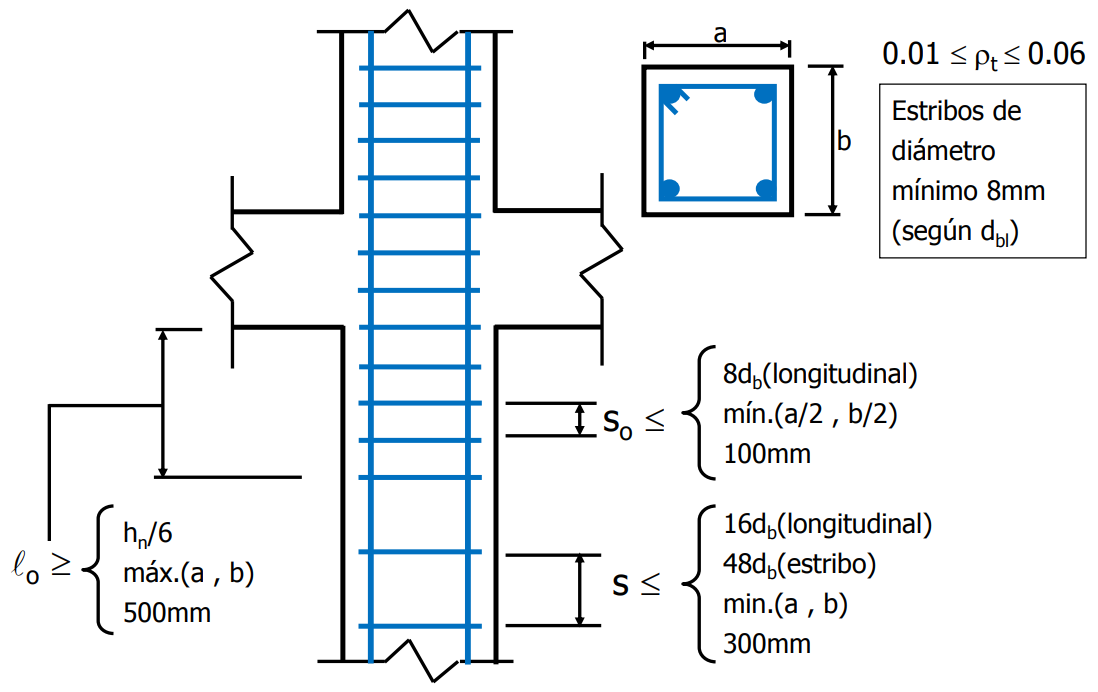
\includegraphics[width=102mm]{IMAGENES/col1.PNG}}\vspace{5mm}
    \subfigure[Sistemas de pórticos o duales]{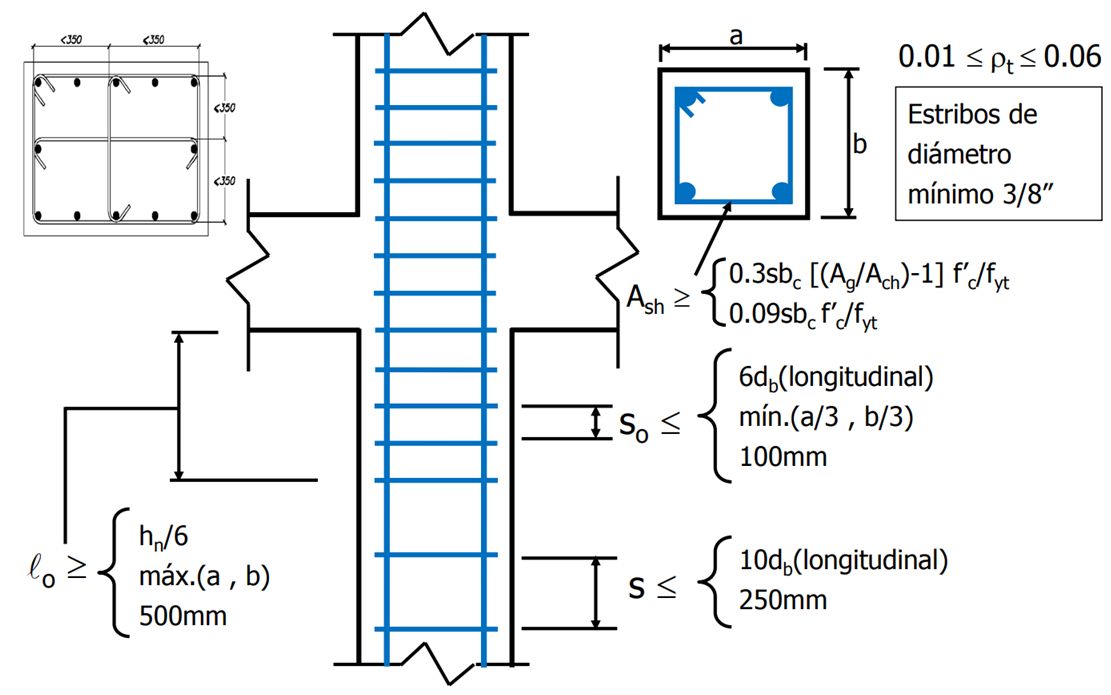
\includegraphics[width=102mm]{IMAGENES/col2.PNG}}
   \caption*{Fuente: \cite{CAPUCP}} 
    \label{reqv}
\end{figure}
\noindent
\textit{Refuerzo transversal mínimo en columnas de pórticos}\\
\begin{align}
A_{sh} &=0.3\; \frac{s\; b_{c}\;f_{c}^{\prime}}{f_{yh}}\left[\left(\frac{A_{g}}{A_{ch}}\right)-1\right]\label{ascolmin} \\
A_{sh} &=0.09\; \frac{s\; b_{c}\; f_{c}^{\prime}}{f_{yh}}\label{ascolmin2}
\end{align}
\noindent Donde:\\
$A_{sh}$: Área de refuerzo transversal (ver figura \ref{atrans})\\
$b_{c}$: es la dimensión del núcleo confinado del elemento normal al refuerzo medida centro a centro del refuerzo de confinamiento\\
$A_{ch}$: es el área del núcleo confinado medida al exterior del refuerzo de confinamiento\\
$A_{g}$: es el área de la sección bruta de la columna\\
$s$: separación del refuerzo transversal\\
$f_{yh}$: Esfuerzo de fluencia del refuerzo transversal
\begin{figure}[h!]
    \centering
    \caption{Área de acero transversal en columnas}
    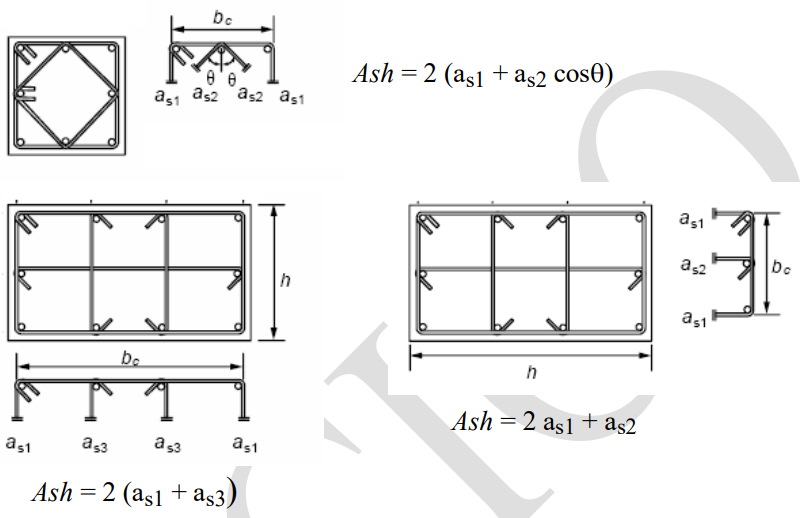
\includegraphics[scale=0.67]{IMAGENES/cc3.PNG}
    \caption*{\small Fuente: \it \cite{E-060}}
    \label{atrans}
\end{figure}
\newpage
\begin{theo}[Art. 21.6.4.1 (c) E-060 :]{thm:ca1}
Cuando la resistencia de diseño del núcleo de la sección transversal del elemento satisface los requisitos de las combinaciones de carga de diseño, incluyendo el efecto sísmico, no es necesario satisfacer la ecuación \ref{ascolmin}.
\end{theo}

\noindent En el presente caso de estudio la altura libre de mayor longitud se encuentra en el primer piso $h_{n}=3.3\;m-0.4\;m=\fpeval{3.3-0.4}\;m$
:\\
La longitud de confinamiento sera el mayor de:
\begin{itemize}
\item $h_{n} / 6= 2.9\;m/6 = 48.3\mathrm{~cm}$
\item $\max (b_{c},h_{c})= 65\mathrm{~cm}$
\item $50 \mathrm{~cm}$
\end{itemize}
La condición (b) es la mas critica por lo tanto se confinara 65cm por encima y por debajo de la luz libre de la columna.\\
La separación en esta longitud sera el menor de:
 \begin{itemize} 
\item $6d_{b}=9.53 \mathrm{~cm}$
\item $\min (b,h)/ 3=10 \mathrm{~cm}$
\item $10 \mathrm{~cm}$
    \end{itemize} 
Se adopta 10cm.\\
La separación fuera de la longitud de confinamiento sera el menor de:
 \begin{itemize} 
\item $10d_{b}=15.88 \mathrm{~cm}$
\item $25 \mathrm{~cm}$
    \end{itemize}
Se adopta 15cm.\\
La resistencia de diseño del núcleo sera:
\FPeval{\ach}{round((\bc-2*\rec)*(\hc-2*\rec),2)}
\FPeval{\pnn}{round(0.8*0.7*(0.85*\fc*(\ach-\Ast)+\Ast*\fy)/1000,2)}
\begin{align*}
    A_{ch}&=\left ( b-2\cdot r_{e} \right )\left ( h-2\cdot r_{e} \right )= \left ( \bc-2\cdot \rec \right )\left ( \hc-2\cdot \rec \right )=\ach \mathrm{~cm^2}\\
    \phi P_{n}&=0,80 \cdot 0,70 \cdot\left[0,85 \cdot \fc \cdot\left(\ach-\Ast\right)+\fy \cdot \Ast\right]=\pnn \mathrm{~ton}
\end{align*}
La capacidad de la columna cuando se pierde el recubrimiento es suficiente para soportar las cargas amplificadas que incluyen sismo, por lo que no es necesario satisfacer la ecuación \ref{ascolmin}.\\
El área de acero transversal requerido por la ecuación \ref{ascolmin2} sera:\\
Dirección del eje fuerte:
\FPeval{\bcc}{round((\bc-2*\rec-\dest),2)}
\FPeval{\hcc}{round((\hc-2*\rec-\dest),2)}
\FPset\sep{10}
\FPeval{\asnif}{round((0.09*\sep*\bcc*\fc/\fy),2)}
\FPeval{\asniff}{round((0.09*\sep*\hcc*\fc/\fy),2)}
\begin{align*}
b_{c}&=b-2\cdot r_{e}-d_{e}=\bc-2\cdot\rec-\dest=\bcc \mathrm{~cm}\\
A_{sh} &=0.09\; \frac{\sep\cdot \bcc\cdot \fc}{\fy}=\asnif\mathrm{~cm^2}
\end{align*}
Dirección del eje débil:
\begin{align*}
b_{c}&=h-2\cdot r_{e}-d_{e}=\hc-2\cdot\rec-\dest=\hcc \mathrm{~cm}\\
A_{sh} &=0.09\; \frac{\sep\cdot \hcc\cdot \fc}{\fy}=\asniff \mathrm{~cm^2}
\end{align*}
\noindent
Por lo tanto se colocaran 4 ramas en la dirección débil por el requisito de la ecuación \ref{ascolmin2}, en la dirección fuerte se colocara 3 ramas por requisito de fuerza cortante. 
\subsubsection{Requisitos adicionales para columnas de sistemas de pórticos o duales}
Según el articulo 21.6.1 estos elementos deben cumplir con:
\FPeval{\limp}{round(0.1*\fc*\Ag/1000,2)}
\begin{enumerate}
\item[] (a): La carga axial amplificada excede $0.1\;f_{c}^{'}\;A_{g}=0.1\cdot\fc\cdot\Ag=\limp\mathrm{~ton}$
\item[] (b): La menor dimensión deber ser mínimamente $B=25 \mathrm{~cm}$
\item[] (c): La relación entre la menor dimensión y la mayor sera menor que $B/L\geq 0.25$
\end{enumerate}
\begin{figure}[hb!]
    \centering
    \caption{Columna de un sistema aporticado o dual}
    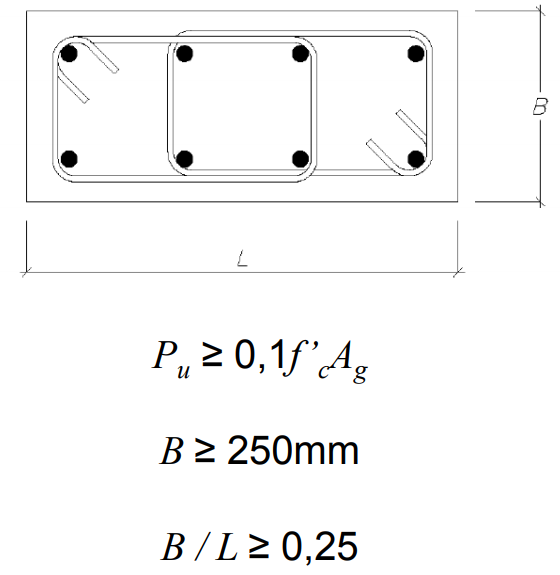
\includegraphics[trim={0 5.5cm 0 0},clip,scale=0.6]{IMAGENES/cc1.PNG}
    %\caption*{\small Fuente: \it \cite{cordova2015}}
    \label{vig}
\end{figure}
\newpage
\noindent
Según la carga axial obtenida, las columnas de los niveles 1 y 2 entrarían en esta categoría.\\
\textit{Resistencia mínima a flexión de las columnas}\\
El articulo 21.6.6.2 requiere que las resistencias a flexión de las columnas en las caras de los nudos deben satisfacer la ecuación (21-1) de la \cite{E-060}:
\begin{align}
\sum M_{nc}\geq 1.2\sum M_{nv}
\end{align}
\noindent Donde:\\
$M_{nc}$: suma de los momentos nominales de flexión de las columnas que llegan al nudo, evaluados en las caras del nudo.   La resistencia a la flexión de la columna debe calcularse para  la  fuerza  axial  amplificada,  consistente  con la  dirección  de  las  fuerzas  laterales consideradas, que conduzca a la resistencia a la flexión más baja.\\
$M_{nv}$: suma de los momentos resistentes nominales a flexión de las vigas que llegan al nudo, evaluados en las caras del nudo.\\
\begin{figure}[h!]
    \centering
    \caption{Criterio columna fuerte-viga débil}
    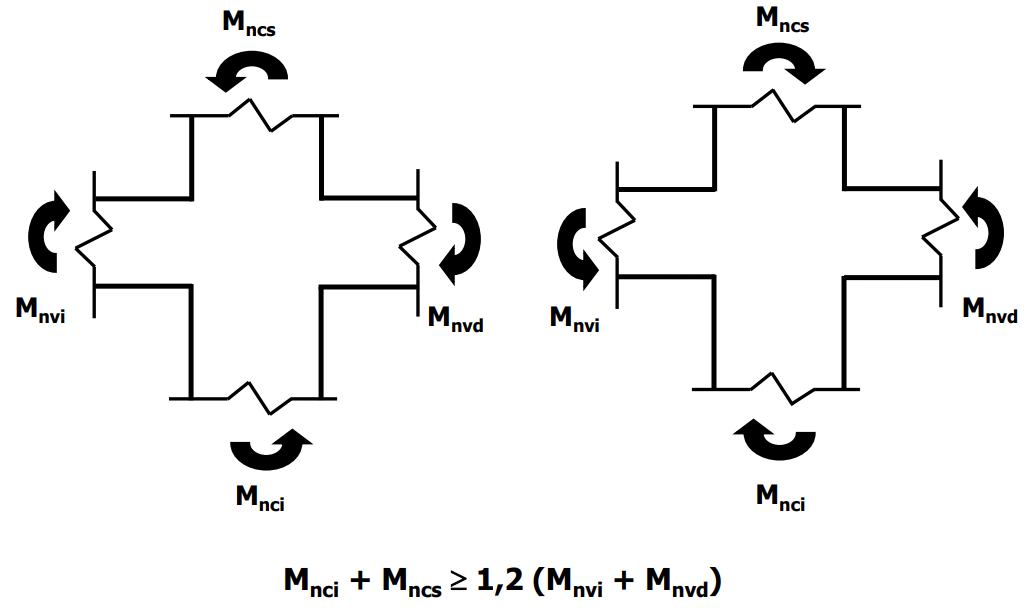
\includegraphics[scale=0.5]{IMAGENES/cc2.PNG}
    %\caption*{\small Fuente: \it \cite{cordova2015}}
    \label{vig}
\end{figure}
\FPset\bsec{25}
\FPset\hsec{40}
\FPeval\asec{round(2*1.98,2)}
\FPeval\dsec{round(\hsec-6,2)}
\FPeval{\mnsec}{round((\asec*\fy*(\dsec-\asec*\fy/(1.7*\fc*\bsec)))/100000,2)}
\FPeval\mnsecd{round(1.2*2*\mnsec,2)}
\noindent La resistencia a la flexión de las vigas secundarias (25x40) que llegan a la columna considerando 2$\phi$5/8" como armado sera:
$$
M_{n}=A_{s}\cdot f_{y}\left ( d-\frac{A_{s}\cdot f_{y}}{1.7\cdot f_{c}^{'}\cdot b} \right )$$
$$
M_{n}=\asec \cdot \fy\left ( \dsec-\frac{\asec\cdot \fy}{1.7\cdot\fc \cdot \bsec} \right )=\mnsec\;\mathrm{~ton.m} 
$$
\FPset\mncol{13.05}
\FPeval\mncoll{round(2*\mncol,2)}
\noindent 
Del diseño por capacidad la menor resistencia de la columna en los pisos 1 y 2 resulta 13.05 ton.m.
\begin{align*}
\sum M_{nc}&\geq 1.2\sum M_{nv}\\
\left ( \mncol+\asnifmncol \right )&\geq 1.2\left ( \mnsec+\mnsec \right )\\
\mncoll \mathrm{~ton.m} &\geq \mnsecd \mathrm{~ton.m}
\end{align*}
\noindent Se cumple el criterio de columna fuerte viga débil.\\
\textit{Refuerzo transversal en nudos}
\begin{theo}[Art. 21.7.3 E-060 :]{thm:ca1}
Dentro  del  nudo  deben  colocarse  estribos  cerrados  de  confinamiento  como refuerzo transversal, tal como lo específica 21.6.4, a menos que dicho nudo esté confinado por elementos estructurales, como lo específica 21.7.3.2.\\
Cuando existan elementos que llegan en los cuatro lados del nudo y el ancho de cada elemento mide por lo menos tres cuartas partes del ancho de la columna, debe disponerse refuerzo transversal igual, por lo menos a la mitad de la cantidad requerida en 21.6.4.1, dentro del peralte del elemento de menor altura. En estos lugares, se permite que el espaciamiento especificado en 21.6.4.2 se  incremente a 150 mm.
\end{theo}
\noindent
\textit{Resistencia a cortante en nudos}\\
Art. 21.7.4: La  resistencia  Vn en  el  nudo  no  debe  ser  mayor  que  las  fuerzas  especificadas  a continuación, para concreto de peso normal:
\begin{flalign}
&\textup{Para nudos confinados en las cuatro caras:}\quad \text{\makebox[7cm]{\dotfill $5.3\sqrt{f_{c}^{\prime}}\;A_{j}$}}&&\\
&\textup{Para nudos confinados en tres caras o en dos caras opuestas:}
\quad \text{\makebox[3.7cm]{\dotfill $4.0\sqrt{f_{c}^{\prime}}\;A_{j}$}}&&\\
&\textup{Para otros casos:} \quad \text{\makebox[11.6cm]{\dotfill $3.2\sqrt{f_{c}^{\prime}}\;A_{j}$}}&&
\end{flalign}
\newpage
Se considera que un elemento (viga) proporciona confinamiento al nudo si al menos las tres cuartas partes de la cara lateral del nudo está cubierta por el elemento que llega al nudo.
\begin{figure}[h!]
    \centering
    \subfigure[Tipos de nudos]{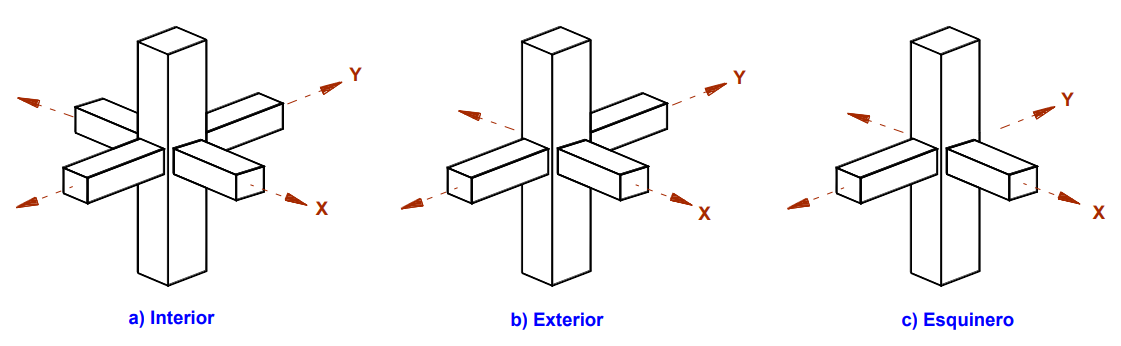
\includegraphics[width=150mm]{IMAGENES/cc6.PNG}}\vspace{10mm}
    \subfigure[Área efectiva del nudo]{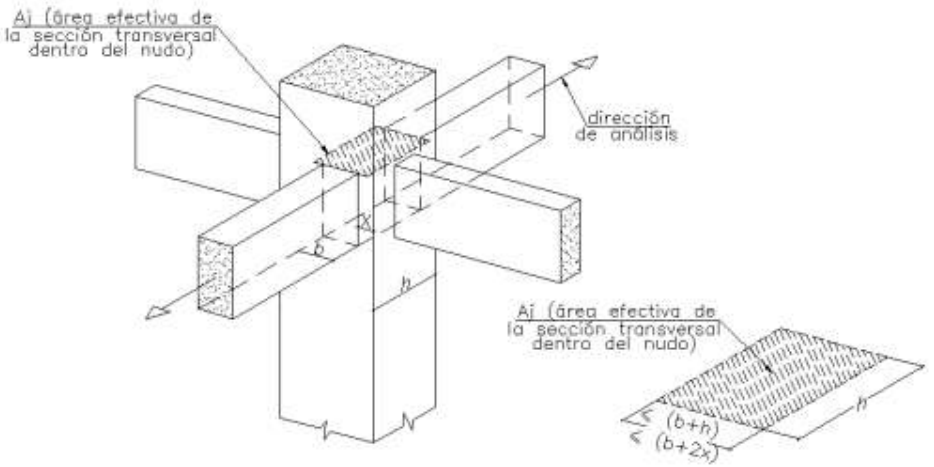
\includegraphics[width=100mm]{IMAGENES/cc4.PNG}}
    \caption{Resistencia a cortante de nudos}
    \label{reqv}
\end{figure}
\newpage
\begin{figure}[ht!]
    \centering
    \subfigure[Equilibrio de fuerzas en el nudo]{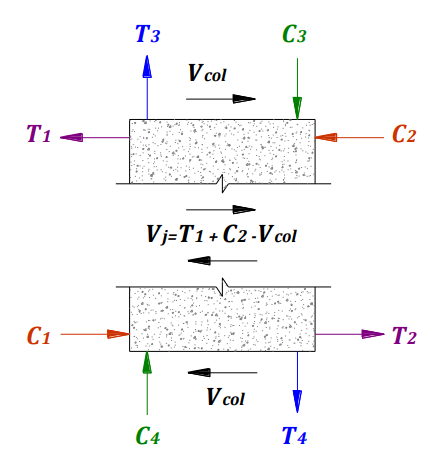
\includegraphics[width=80mm]{IMAGENES/cc5.PNG}}\hspace{10mm}
    \subfigure[Cortante en columna]{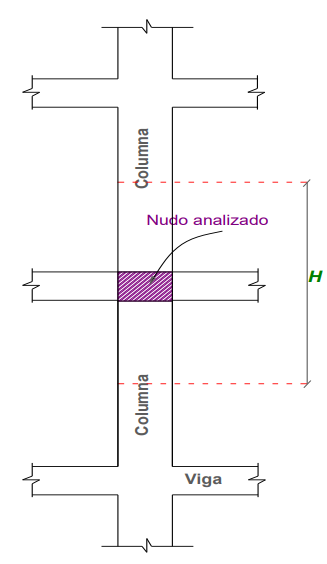
\includegraphics[width=60mm]{IMAGENES/cc7.PNG}}
    \caption{Resistencia a cortante de nudos}
    \label{reqn}
\end{figure}
\textit{Refuerzo transversal en nudos}
\begin{theo}[Area efectiva del nudo Art. 21.7.4.1 E-060 :]{thm:ca1}
$A_{j}$ es el área efectiva de la sección transversal dentro del nudo en la dirección de análisis, calculada  como  el  producto  de  la  profundidad  del  nudo  por su  ancho  efectivo. La profundidad del nudo es la dimensión total de la columna en la dirección de análisis. El ancho efectivo del nudo es el ancho total de la columna, excepto que cuando la viga llega a una columna más ancha que ésta, el ancho efectivo del nudo no debe exceder el menor de (a) y (b):
\begin{enumerate}
\item[] (a): el ancho de la viga más la profundidad del nudo.  Si el ancho difiere a ambos lados de la columna, se utilizará el promedio de ellos.
\item[] (b): dos veces la distancia del eje longitudinal de la viga al borde más cercano de la columna
\end{enumerate}
\end{theo}
\noindent 
En este caso se trata de un columna exterior, por tanto la profundidad del nudo es igual al ancho de la columna \bc cm y teniendo en cuenta que el ancho de la viga es de \bsec cm el ancho efectivo sera el menor de:
\FPeval{\aa}{round(\bsec+\bc,0)}
\FPeval{\xx}{round(0.5*\bsec,2)}
\FPeval{\bb}{round(\bsec+\xx*2,0)}
\begin{enumerate}
\item[] (a): \bsec+\bc=\aa cm
\item[] (b): \bsec+$2x$=\bsec+\xx=\bb cm
\end{enumerate}
\FPmin\cc{\aa}{\bb}
El área efectiva y la resistencia a cortante del nudo respectivamente sera:
\FPeval{\aj}{round(\cc*\bc,2)}
\FPeval{\vnu}{round(0.5*4*\rc*\aj/1000,2)}
\begin{align*}
A_{j}&=\cc\cdot\bc=\aj \mathrm{~cm^2}\\
\phi V_{n}&=0.85\cdot4.0\cdot\sqrt{\fc}\cdot\aj=\vnu \mathrm{~ton}
\end{align*}
\noindent La cortante en la columna producto de la fluencia de las vigas sera:
\FPset\hcol{2.4}
\FPeval\vcoln{round(1.25*2*\mnsec/\hcol,2)}
\begin{align}
V_{col}&=2\;\frac{M_{pi}+M_{pd}}{H}\\
V_{col}&=2\cdot\frac{1.25\cdot2\cdot\mnsec}{\hcol}=\vcoln\notag \mathrm{~ton}
\end{align}
\noindent
Donde:\\
$M_{pi},M_{pd}$: Momentos de vigas a cada lado del nudo para 1.25$f_{y}$ (Art. 21.7.2.1)\\
$H$: Altura entre puntos de inflexión de la columna (ver figura \ref{reqn})\\
\noindent La cortante producida en el nudo según 21.7.4.3 sera:
\FPeval{\vnuu}{round(1.25*2*\asec*\fy/1000-\vcoln,2)}
\begin{align}
V_{u}&=1.25\left ( A_{s1}+A_{s2} \right )f_{y}-V_{col}\\
V_{u}&=1.25\left ( \asec+\asec \right )\cdot \fy-\vcoln \mathrm{~ton}=\vnuu\mathrm{~ton}\notag
\end{align}
\noindent Se cumple con $\phi V_{n}\geq V_{u}$.
